\RequirePackage[l2tabu,orthodox]{nag}
\documentclass[headsepline,footsepline,footinclude=false,oneside,fontsize=11pt,paper=a4,listof=totoc,bibliography=totoc,DIV=12]{scrbook} % one-sided

\PassOptionsToPackage{table,svgnames,dvipsnames}{xcolor}

\usepackage[utf8]{inputenc}
\usepackage[T1]{fontenc}
\usepackage[sc]{mathpazo}
\usepackage[ngerman,english]{babel} % english is the same as american or USenglish
\usepackage[autostyle]{csquotes}
\usepackage[%
  backend=biber,
  url=true,
  style=numeric, % alphabetic, numeric
  sorting=none, % default == nty, https://tex.stackexchange.com/questions/51434/biblatex-citation-order
  maxnames=4,
  minnames=3,
  maxbibnames=99,
  giveninits,
  uniquename=init]{biblatex} % TODO: adapt citation style
\usepackage{graphicx}
\usepackage{scrhack} % necessary for listings package
\usepackage{listings}
\usepackage{lstautogobble}
\usepackage{tikz}
\usepackage{pgfplots}
\usepackage{pgfplotstable}
\usepackage{booktabs} % for better looking table creations, but bad with vertical lines by design (package creator despises vertical lines)
\usepackage[final]{microtype}
\usepackage{caption}
\usepackage[hidelinks]{hyperref} % hidelinks removes colored boxes around references and links
\usepackage{ifthen} % for comparison of the current language and changing of the thesis layout
\usepackage{pdftexcmds} % string compare to work with all engines
\usepackage{paralist} % for condensed enumerations or lists
\usepackage{subfig} % for having figures side by side
\usepackage{siunitx} % for physical accurate units and other numerical presentations
\usepackage{multirow} % makes it possible to have bigger cells over multiple rows in a table
\usepackage{array} % different options for table cell orientation
\usepackage{makecell} % allows nice manual configuration of cells with linebreaks in \thead and \makecell with alignments
\usepackage{pdfpages} % for including multiple pages of pdfs
\usepackage{adjustbox} % can center content wider than the \textwidth
\usepackage{tablefootnote} % for footnotes in tables as \tablefootnote
\usepackage{threeparttable} % another way to add footnotes as \tablenotes with \item [x] <your footnote> after setting \tnote{x} 


% https://tex.stackexchange.com/questions/42619/x-mark-to-match-checkmark
\usepackage{amssymb}% http://ctan.org/pkg/amssymb
\usepackage{pifont}% http://ctan.org/pkg/pifont
\newcommand{\cmark}{\ding{51}}%
\newcommand{\xmark}{\ding{55}}%


\usepackage[acronym,xindy,toc]{glossaries} % TODO: include "acronym" if glossary and acronym should be separated
\makeglossaries
\loadglsentries{pages/glossary.tex} % important update for glossaries, before document


\bibliography{bibliography}

\setkomafont{disposition}{\normalfont\bfseries} % use serif font for headings
\linespread{1.05} % adjust line spread for mathpazo font

% Add table of contents to PDF bookmarks
\BeforeTOCHead[toc]{{\cleardoublepage\pdfbookmark[0]{\contentsname}{toc}}}

% Define TUM corporate design colors
% Taken from http://portal.mytum.de/corporatedesign/index_print/vorlagen/index_farben
\definecolor{TUMBlue}{HTML}{0065BD}
\definecolor{TUMSecondaryBlue}{HTML}{005293}
\definecolor{TUMSecondaryBlue2}{HTML}{003359}
\definecolor{TUMBlack}{HTML}{000000}
\definecolor{TUMWhite}{HTML}{FFFFFF}
\definecolor{TUMDarkGray}{HTML}{333333}
\definecolor{TUMGray}{HTML}{808080}
\definecolor{TUMLightGray}{HTML}{CCCCC6}
\definecolor{TUMAccentGray}{HTML}{DAD7CB}
\definecolor{TUMAccentOrange}{HTML}{E37222}
\definecolor{TUMAccentGreen}{HTML}{A2AD00}
\definecolor{TUMAccentLightBlue}{HTML}{98C6EA}
\definecolor{TUMAccentBlue}{HTML}{64A0C8}

% Settings for pgfplots
\pgfplotsset{compat=newest}
\pgfplotsset{
  % For available color names, see http://www.latextemplates.com/svgnames-colors
  cycle list={TUMBlue\\TUMAccentOrange\\TUMAccentGreen\\TUMSecondaryBlue2\\TUMDarkGray\\},
}

% Settings for lstlistings

% Use this for basic highlighting
\lstset{%
  basicstyle=\ttfamily,
  columns=fullflexible,
  autogobble,
  keywordstyle=\bfseries\color{TUMBlue},
  stringstyle=\color{TUMAccentGreen}
}

% use this for C# highlighting
% %\setmonofont{Consolas} %to be used with XeLaTeX or LuaLaTeX
% \definecolor{bluekeywords}{rgb}{0,0,1}
% \definecolor{greencomments}{rgb}{0,0.5,0}
% \definecolor{redstrings}{rgb}{0.64,0.08,0.08}
% \definecolor{xmlcomments}{rgb}{0.5,0.5,0.5}
% \definecolor{types}{rgb}{0.17,0.57,0.68}

% \lstset{language=[Sharp]C,
% captionpos=b,
% %numbers=left, % numbering
% %numberstyle=\tiny, % small row numbers
% frame=lines, % above and underneath of listings is a line
% showspaces=false,
% showtabs=false,
% breaklines=true,
% showstringspaces=false,
% breakatwhitespace=true,
% escapeinside={(*@}{@*)},
% commentstyle=\color{greencomments},
% morekeywords={partial, var, value, get, set},
% keywordstyle=\color{bluekeywords},
% stringstyle=\color{redstrings},
% basicstyle=\ttfamily\small,
% }

% Settings for search order of pictures
\graphicspath{
    {logos/}
    {figures/}
}

% Set up hyphenation rules for the language package when mistakes happen
\babelhyphenation[english]{
an-oth-er
ex-am-ple
}

% Decide between
%\newcommand{\todo}[1]{\textbf{\textsc{\textcolor{TUMAccentOrange}{(TODO: #1)}}}} % for one paragraph, otherwise error!
%\newcommand{\done}[1]{\textit{\textsc{\textcolor{TUMAccentBlue}{(Done: #1)}}}} % for one paragraph, otherwise error!
% and
\newcommand{\todo}[1]{{\bfseries{\scshape{\color{TUMAccentOrange}[(TODO: #1)]}}}} % for multiple paragraphs
\newcommand{\done}[1]{{\itshape{\scshape{\color{TUMAccentBlue}[(Done: #1)]}}}} % for multiple paragraphs
% for error handling of intended behavior in your latex documents.

\newcommand{\tabitem}{~~\llap{\textbullet}~~}

\newcolumntype{P}[1]{>{\centering\arraybackslash}p{#1}} % for horizontal alignment with limited column width
\newcolumntype{M}[1]{>{\centering\arraybackslash}m{#1}} % for horizontal and vertical alignment with limited column width
\newcolumntype{L}[1]{>{\raggedright\arraybackslash}m{#1}} % for vertical alignment left with limited column width
\newcolumntype{R}[1]{>{\raggedleft\arraybackslash}m{#1}} % for vertical alignment right with limited column width

\newcommand*{\getUniversity}{Technische Universität München}
\newcommand*{\getFaculty}{Department of Informatics}
\newcommand*{\getTitle}{Developing a Scalable, Secure, and Privacy-preserving Platform for Collection, Aggregation, and Analysis of Mobility Data}
\newcommand*{\getTitleGer}{Entwicklung einer skalierbaren, sicheren, privatsphäre-erhaltenden Plattform zur Sammlung, Aggregation und Analyse von Mobilitätsdaten}
\newcommand*{\getAuthor}{Dinh Le Khanh Duy}
\newcommand*{\getDoctype}{Master's Thesis in Informatics}
\newcommand*{\getSupervisor}{Prof. Dr.-Ing. Jörg Ott}
\newcommand*{\getAdvisor}{Doan Trinh Viet}
\newcommand*{\getSubmissionDate}{15.03.2020}
\newcommand*{\getSubmissionLocation}{Munich}

\usepackage{multicol}
\usepackage{listings}
\usepackage{xcolor}
 
\definecolor{codegreen}{rgb}{0,0.6,0}
\definecolor{codegray}{rgb}{0.5,0.5,0.5}
\definecolor{codepurple}{rgb}{0.58,0,0.82}
\definecolor{backcolour}{rgb}{0.95,0.95,0.92}
 
\lstdefinestyle{mystyle}{
    backgroundcolor=\color{backcolour},   
    commentstyle=\color{codegreen},
    keywordstyle=\color{magenta},
    numberstyle=\tiny\color{codegray},
    stringstyle=\color{codepurple},
    basicstyle=\ttfamily\footnotesize,
    breakatwhitespace=false,         
    breaklines=true,                 
    captionpos=b,                    
    keepspaces=true,                 
    numbers=left,                    
    numbersep=5pt,                  
    showspaces=false,                
    showstringspaces=false,
    showtabs=false,                  
    tabsize=2
}
\lstset{style=mystyle}

\begin{document}

%\selectlanguage{ngerman}
\selectlanguage{english}

% Set page numbering to avoid "destination with the same identifier has been already used" warning for cover page.
% (see https://en.wikibooks.org/wiki/LaTeX/Hyperlinks#Problems_with_Links_and_Pages).
\pagenumbering{alph}
\begin{titlepage}
  % HACK for two-sided documents: ignore binding correction for cover page.
  % Adapted from Markus Kohm's KOMA-Script titlepage=firstiscover handling.
  % See http://mirrors.ctan.org/macros/latex/contrib/koma-script/scrkernel-title.dtx,
  % \maketitle macro.
  \oddsidemargin=\evensidemargin\relax
  \textwidth=\dimexpr\paperwidth-2\evensidemargin-2in\relax
  \hsize=\textwidth\relax

  \centering

  \IfFileExists{logos/tum.pdf}{%
    
\includegraphics[height=20mm]{logos/tum.pdf}
  }{%
    \vspace*{20mm}
  }

  \vspace{5mm}
  {\huge\MakeUppercase{\getFaculty{}}}\\

  \vspace{5mm}
  {\large\MakeUppercase{\getUniversity{}}}\\

  \vspace{20mm}
  {\Large \getDoctype{}}

  \vspace{15mm}
  \makeatletter
  \ifthenelse{\pdf@strcmp{\languagename}{english}=0}
  {\huge\bfseries \getTitle{}}
  {\huge\bfseries \getTitleGer{}}
  \makeatother

  \vspace{15mm}
  {\LARGE \getAuthor{}}

  \IfFileExists{logos/faculty.png}{%
    \vfill{}
    
\includegraphics[height=20mm]{logos/faculty.png}
  }{}
\end{titlepage}


\frontmatter{}

\begin{titlepage}
  \centering

  \IfFileExists{logos/tum.pdf}{%
    
\includegraphics[height=20mm]{logos/tum.pdf}
  }{%
    \vspace*{20mm}
  }

  \vspace{5mm}
  {\huge\MakeUppercase{\getFaculty{}}}\\

  \vspace{5mm}
  {\large\MakeUppercase{\getUniversity{}}}\\

  \vspace{20mm}
  {\Large \getDoctype{}}

  \makeatletter
  \vspace{15mm}
  \ifthenelse{\pdf@strcmp{\languagename}{english}=0}
  {
  {\huge\bfseries \getTitle{}}

  \vspace{10mm}
  {\huge\bfseries \foreignlanguage{ngerman}{\getTitleGer{}}}
  }
  {
  {\huge\bfseries \getTitleGer{}}

  \vspace{10mm}
  {\huge\bfseries \foreignlanguage{english}{\getTitle{}}}
  }
  \makeatother

  \vspace{15mm}
  \begin{tabular}{l l}
    Author:          & \getAuthor{} \\
    Supervisor:      & \getSupervisor{} \\
    Advisor:         & \getAdvisor{} \\
    Submission Date: & \getSubmissionDate{} \\
  \end{tabular}

  \IfFileExists{logos/faculty.png}{%
    \vfill{}
    
\includegraphics[height=20mm]{logos/faculty.png}
  }{}
\end{titlepage}

\cleardoublepage{}

\thispagestyle{empty}
\vspace*{0.8\textheight}
\noindent
\makeatletter
\ifthenelse{\pdf@strcmp{\languagename}{english}=0}
{I confirm that this \MakeLowercase{\getDoctype{}} is my own work and I have documented all sources and material used.}
{Ich versichere, dass ich diese \getDoctype{} selbstständig verfasst und nur die angegebenen Quellen und Hilfsmittel verwendet habe.}
\makeatother

\vspace{15mm}
\noindent
\getSubmissionLocation{}, \getSubmissionDate{} \hspace{50mm} \getAuthor{}

\cleardoublepage{}

\chapter{\abstractname}

%TODO: write abstract

blablablbalblalbalbal

\microtypesetup{protrusion=false}
\tableofcontents{}
\microtypesetup{protrusion=true}

\mainmatter{}

% !TeX root = ../main.tex
% Add the above to each chapter to make compiling the PDF easier in some editors.

\chapter{Introduction}\label{chapter:introduction}
\section{Motivation}

There are currently around 7.7 billion people living on earth with a declining growth rate at currently 1.1 percent per year. The UN is predicting that the population growth is going to be sinking steadily in the next decades, but despite that, the population is projected to increase until 2100. They estimate that the earth will hit approximately 10.9 billion at the end of the century, according to their diagram \ref{fig:population}.

\begin{figure}[htpb]
  \centering
  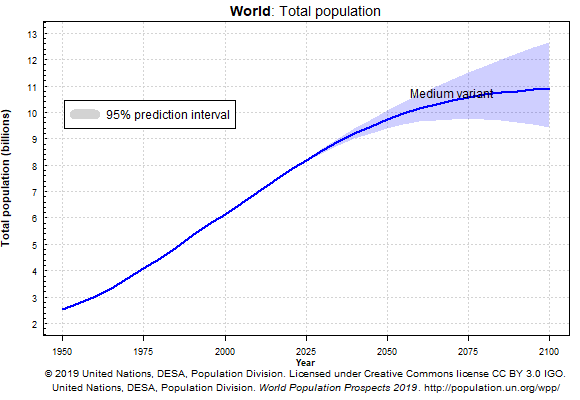
\includegraphics[width=0.8\textwidth]{figures/population.png}
  \caption{Projections for population growth this century} \label{fig:population}
\end{figure}

% Todo: \cite[UN Population Facts] 

Big cities and metropoles around the globe are inevitably growing denser year by year. According to the United Nations, urban areas around the globe have been experiencing an influx of people since the start of industrialization. While the same can be said for rural areas because of the general growth rate of the population, the increase in people moving into big cities is much higher compared to the countryside.
% Todo: \cite[Population Growth in the World's Largest Cities]
% Todo: \cite[UN Interactive Data: Annual Urban Population at Mid-Year (thousands)]
% Todo: \cite[UN Interactive Data: Annual Rural Population at Mid-Year (thousands)]
% Todo: \cite[UN Interactive Data: Average Annual Rate of Change of the Urban Population (percent)]
% Todo: \cite[UN Interactive Data: Average Annual Rate of Change of the Rural Population (percent)]
Depending on how certain factors evolve, such as climate change, autonomous driving, and other technology and politics, it could decelerate or even accelerate growth.

To solve issues stemming from the increased demand in housing, traffic, and infrastructure, urban planning is one of the most important tools. Improving traffic control requires knowledge of the traffic flow and inefficiencies that are causing traffic jams. Knowing local population trends, movement patterns, and other factors could benefit the planning of housing and energy infrastructure. There are only a handful of companies that hold the monopoly on the much-required data, but acquiring them is expensive and can cause problems with data protection laws. Publicizing the information without anonymizing it, severely infringes on the privacy of the originator of the data. But the sole act of anonymizing the data is often not enough. The use of inference attacks may make it possible to associate data and re-identify the individual, as L. Sweeney has proven.
% Todo: \cite[k-Anonymity/ A Model for Protecting Privacy]

To solve some of the issues, we can leverage the widespread availability of portable computing power, and create a platform that provides the data on a need-to-know basis. Today, most smartphones are equipped with several sensors, including a GPS sensor, pedometer, and accelerometer, which can be used to collect a wide variety of mobility data. Many applications are already utilizing those sensors to implement location-based services and games; for instance, Google Maps, Uber, and Pokemon GO. But there has been a lot of controversy around products of that kind. "If you're not paying, you're the product" is a quote that is often cited around data-driven applications.
% Todo: \cite[https://www.nytimes.com/2018/04/08/us/facebook-users-data-harvested-cambridge-analytica.html]
% Todo: \cite[https://www.ted.com/talks/zeynep_tufekci_we_re_building_a_dystopia_just_to_make_people_click_on_ads]
% Todo: \cite[https://arstechnica.com/tech-policy/2018/04/steve-wozniak-leaves-facebook-the-profits-are-all-based-on-the-users-info/]
% Todo: \cite[https://gadgets.ndtv.com/internet/news/tim-cook-to-google-users-youre-not-the-customer-youre-the-product-594242]
It applies to a lot of free services offered in exchange for your data. Google Maps, for example, provides a free navigation service, while collecting your sensory data, such as GPS and accelerometer, staying informed about traffic information. Facebook provides a free social media platform for people to connect, in turn, using collected data to sell targeted advertising.

How they use your data is not in your control. So publicizing big anonymous data sets has its limits, and data collection itself is a hot topic in today's media. 

\section{Research Questions}
We try to find a balance between the usability of data, the privacy preservation of the data collecting user, and the trust between the servers and mobile devices.
\subsection*{RQ1: What are the benefits and drawbacks in Simon van Endern's architecture?}
We take a look at Simon van Endern's original idea and implemented architecture. We investigate both the advantages and disadvantages of his idea in regards to scalability, security, and privacy.
% Todo: Something about weak points.
\subsection*{RQ2: What improvements are possible?}
His work shows a minimal viable product on which we can expand further. We search for possible ways to improve on his architecture and explore possible aggregations.
\subsection*{RQ3: Do the raw values for steps and activities infringe on privacy?}
As Simon van Endern has shown, mean values expose less private information. We want to take a look into the raw data that makes up the mean values and analyze the privacy concerns regarding the distribution of the step values and activities values for the participants and if they can  be used to link to other data.
\subsection*{RQ4: Is it possible to query for more accurate location data while preserving privacy?}
Related work has shown that location data are very susceptible to leaking private information. We look into methods to disassociate the mobility data with the individual to provide anonymity while maintaining statistical relevance.
% Todo: about location tracking and spacial cloaking
\subsection*{RQ5: Can we use the current state of P2P technology to remove intermediate third parties?}
There have been a lot of advancements in direct communication frameworks, and we look into possible SDKs that can be leveraged to implement and enable a more decentralized or distributed architecture.

\section{Contributions}

We will reexamine the results found by Simon van Endern, and we will expand on his original idea while focusing on the scalability of the crowdsourcing platform and the privacy analysis of aggregation for more specific mobility data.
% Todo: \cite[Simon van Endern]
% Todo: write more content

First, we will review related work concerning risks and solutions to sensitive data and pertinent anonymization techniques. After that, we will propose our approach to architecture to solve the mentioned problems. In chapter 4, we explain the details of our implementation and decisions. The next chapter documents our field test setup and evaluates our results. Finally, we draw a conclusion on our work and discuss further possible improvements and show how the project can be reproduced.

% !TeX root = ../main.tex
% Add the above to each chapter to make compiling the PDF easier in some editors.

\chapter{Related Work}\label{chapter:relatedwork}
\section{Risks}
While working with sensitive data, we have to assess multiple attack vectors before we can take action. We compile possible attack vectors and how they could be solved.

\subsection{Risks of centralization}
Because of efficiency, centralized information systems have always been a go-to infrastructure. The advantages of simple deployment, ease of maintenance, and less bureaucracy will always be an incentive for big companies and governments to consider it. In 1965, the US Social Science Research Council \cite{lawreview} proposed a National Data Center to store all data in a central location for statistical data analysis. Still, in the end, the plans for the system were shot down because of the lack of privacy protection.

Today, many big tech companies are collecting data about their users and storing them in central databases. Nevertheless, centralization has a fatal flaw in protecting privacy. According to Stolpe \cite{DBLP:journals/sigkdd/Stolpe16}, the collection of sensitive data in one location poses a high risk to their originator.

Centralized databases that store private information are one of the weak points that have been under constant attack for years. After an analysis by RiskBased Security \cite{riskbasedsecurity}, they determined that in the first three quarters of 2019, there have been over 5000 data breaches, with almost 8 billion records exposed, 33\% more compared to the number reported in the first nine months of the previous year. Around 10\% of those breaches originated from the inside, such as accidental leaks and intentional publications.

The vulnerability of central databases makes private data stored prone to attacks from inside, as well as outside.

\subsection{Reconstruction, linkage and tracing attacks}
The first reaction to those data breaches would naturally be to de-identify the data. If we do that by stripping away all sensitive information, making the data set pseudonymous, the risk of private data leaking remains, which can be exploited by reconstruction, linkage, and tracing attacks. The most severe problem is the danger of re-identification \cite{reidentification}\cite{DBLP:journals/midm/EmamBTNJV11}\cite{DBLP:journals/midm/DankarENR12}.
It enables adversaries to deduce the identity of an individual using other publicly available data sets or auxiliary knowledge. 
In her work, Sweeney \cite{DBLP:journals/ijufks/Sweene02} was able to re-identify former Massachusetts governor William Weld by linking medical records from the Group Insurance Commission and the voter registration list.

The goal of reconstruction is to determine sensitive data from a data set that has been generalized or suppressed using publicly available information \cite{DBLP:journals/fttcs/DworkR14}\cite{exposed}. Lacharite\'e \cite{DBLP:conf/sp/LachariteMP18} has proven that efficient reconstruction attacks are very well possible, given a dense data set.
 
Tracing, on the other hand, is the ability to identify if an individual is present in a data set or not \cite{exposed}. It can expose information, which has previously been unknown. Homer et al. \cite{dna} showed how they were able to determine the presence or absence of a target in their genome-wide association study.

\subsection{Risks of location tracking}
In regards to location data, the ability to infer the home and work location poses both risks for privacy and life and limb. Research \cite{DBLP:conf/pervasive/Krumm07}\cite{DBLP:journals/corr/abs-1901-00897}\cite{DBLP:conf/pervasive/GolleP09} has shown that it is possible to track individuals, deduce their home address and even their workplace using historical location data.
Location data is also able to hold more information than just spatial and temporal data. It is possible to associate a spatial location with other sensitive information. For example, the attendance of a political rally can tell an adversary about the political affiliation, or tracking someone to a specialized clinic could expose additional medical data.
Besides, being able to analyze the movement pattern and predict the presence of people in a particular location may put their lives in danger. Being able to determine the presence of people in their homes or their absence might enable someone to break in and rob their house.

\section{Countermeasures}
To implement a secure platform that is less vulnerable to the problems proposed in the sections above, we look into methods and design decisions to prevent them.
\subsection{Distribution and decentralization}
When the Advanced Research Projects Agency Network (ARPANET) implemented the prototype of the internet in 1969, it was a decentralized network of computers scattered across the United States. With the adoption of the TCP/IP in 1982, it became the internet, an interconnected network of networks as we have today \cite{DBLP:books/daglib/0006297}.
In 1989, Tim Berners-Lee introduced the world wide web as a read-only means of accessing information from other computers, and the commercialization turned it into the centralized web we know today. 

The dangers of data breaches can originate from outside the companies as well as inside, and their cause range from poorly implemented security and lax security policies to human error \cite{riskbasedsecurity}.
Figure \ref{fig:comparison} depicts two alternatives in place of a centralized architecture: distributed and decentralized.

\begin{figure}[htpb]
  \centering
  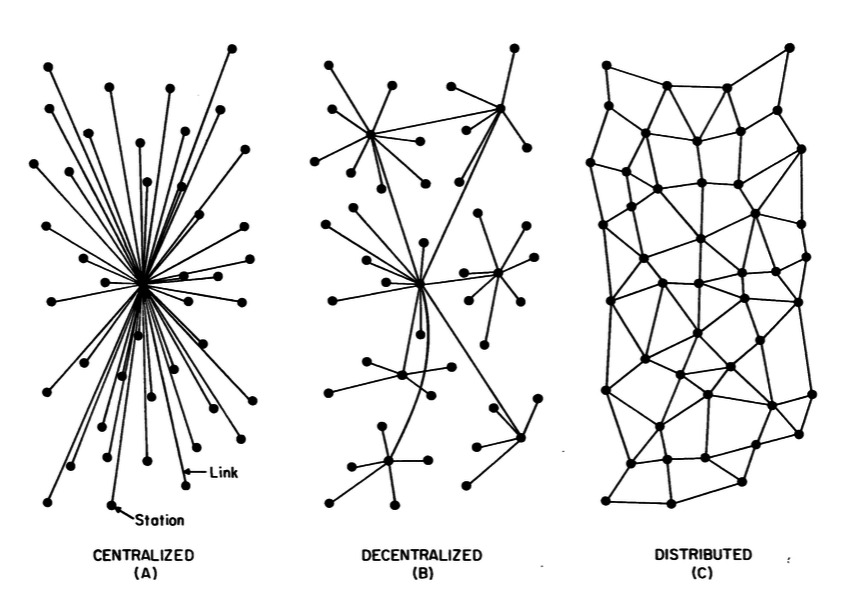
\includegraphics[width=0.8\textwidth]{figures/comparison.jpg}
  \caption{Illustration of a centralized, distributed and decentralized architecture \cite{distributed}} 
  \label{fig:comparison}
\end{figure}

In the last decade, we have seen a rise in attempts to reorganize the internet. This trend amassed attention in 2009 when the creator under the pseudonym Satoshi Nakamoto  \cite{bitcoin} created Bitcoin, "A Peer-to-Peer Electronic Cash System" leveraging blockchain technology, followed by the Ethereum \cite{ethereum} platform in 2013.
The goal of decentralization is the separation of power from a single instance. In our case, it would be to take away control from monopolies over our data. 

One of the protocols that arose from this niche is the InterPlanetary File System (IPFS)\cite{DBLP:journals/corr/Benet14}. IPFS is a peer-to-peer hypermedia protocol to make the web more decentralized and distributed. A node can upload a file, and every file and its blocks generate a cryptographic hash, making it content addressable. Requesting a file will search the network for nodes that store it, and the nodes that have it will provide.

Distribution takes decentralization a step further by eliminating the central control by giving all instances the same amount of power. Using distributed storage, in place of a centralized database, removes the single point of vulnerability and lowers the effort-to-reward balance and thus might deter malicious actors from trying to steal data.

\subsection{Homomorphic encryption}
Conventionally, encryption methods do not provide anonymity. However, one could argue that, in a way, anonymity is provided when the data is not readable or accessible. If an adversary manages to steal a data set while it is still encrypted, they will not be able to infer identity or any additional information, unless they are able to decrypt it beforehand. 

Homomorphic encryption enables the arithmetic operations on an encrypted data set. They are separated into three categories \cite{DBLP:journals/corr/abs-1812-02428}:
\begin{itemize}
    \item \textbf{Fully Homomorphic Encryption (FHE)} allows multiple arbitrary operations, but has a lot of overhead and thus is computationally expensive.
    \item \textbf{Somewhat Homomorphic Encryption (SWHE)} supports only selected operations to a limited number of times and is computationally more feasible.
    \item \textbf{Partially Homomorphic Encryption (PHE)} enables one type of operation any number of times.
\end{itemize}

It protects the data set from intermediate parties, making them unable to derive private data, while still making it possible to work on it. We will look into possible implementations and figure out if this encryption scheme is feasible in a mobile environment.

\subsection{k-Anonymity}
Sweeney \cite{DBLP:journals/ijufks/Sweene02} has shown that anonymous data sets are not as anonymous as they seem. Quasi-identifiers, an identifier or a combination of non-identifying attributes, still enable malicious actors to link individuals back to their data. As one of the possible countermeasures to this problem, she proposes k-anonymity. This is achieved when every query for quasi-identifier returns at least k results. A quasi-identifier, such as ZIP code, birth date, or sex, can be used to link with external data sources to create new identifiers. For this, Samarati \cite{samarati} and Sweeney \cite{DBLP:journals/ijufks/Sweene02} suggest the use of generalization and suppression.

Former is realized by expanding specific attributes into ranges. For instance, instead of assigning the real age, an age range is substituted, resulting in a loss of accuracy, but a higher degree of anonymity. For the latter, there are two methods of suppression. Attribute suppression removes attributes from the data set, reducing the number of possible quasi-identifiers by lowering the number of possible combinations. In contrast, record suppression, on the other hand, deletes entire entries in the data set to take out unique entries that do not meet the criteria of k-anonymity \cite{singapore}.

\subsection{Differential privacy}
In 2006, Dwork \cite{DBLP:conf/icalp/Dwork06} proposed a mathematical definition for differential privacy. It is used to prevent statistical databases from leaking private information. It is a compelling definition that is able to guarantee privacy. An algorithm is differential private as long as it prevents tracing attacks, meaning that output does not show signs of a particular individual is present in it or not. Removing an entry in the data set would not reflect in the resulting queries.
Both Google \cite{erlingsson_2014} and Apple \cite{apple} have implemented differential privacy into their data collection methods.

Differential privacy guarantees three qualities:
\begin{itemize}
    \item All data about an individual in the database is protected even if the adversary manages to learn auxiliary information about all other entries in the data set.
    \item Two differently differential private data sets can be combined, and the resulting data set is still differential private.
    \item It is possible to quantify the loss of privacy and information gained by the malicious actor.
    \item It can be applied to groups.
\end{itemize}

Noise is added to the data to achieve differential privacy,  but replay attacks might be able to reveal actual values. To avoid this, the default noise function used is the Laplacian mechanism or exponential mechanism \cite{DBLP:journals/fttcs/DworkR14}. The noise function also has to be modified to the extent of the sensitivity of the data set. That is the maximum value a single entry in the data set can change the query. For example, a query for the count of true and false answers; the sensitivity is one as the removal of one participant only removes one response of true or false. Nevertheless, the higher the sensitivity, the greater the noise that has to be added to the data to guarantee privacy, which in subsequently makes the data less accurate. The noise can be added either on the aggregation of the user data or on the aggregated data itself.

\subsubsection{Global Differential Privacy}
If the noise function is applied to the entire aggregated raw data set, it is called global differential privacy. It works by using a noise function on the result of a query, as depicted in Figure \ref{fig:global_diff}. The advantage of this model is that the resulting data set is still very accurate, but on the downside, the whole raw data set has to be available to use this function.

\begin{figure}[htpb]
  \centering
  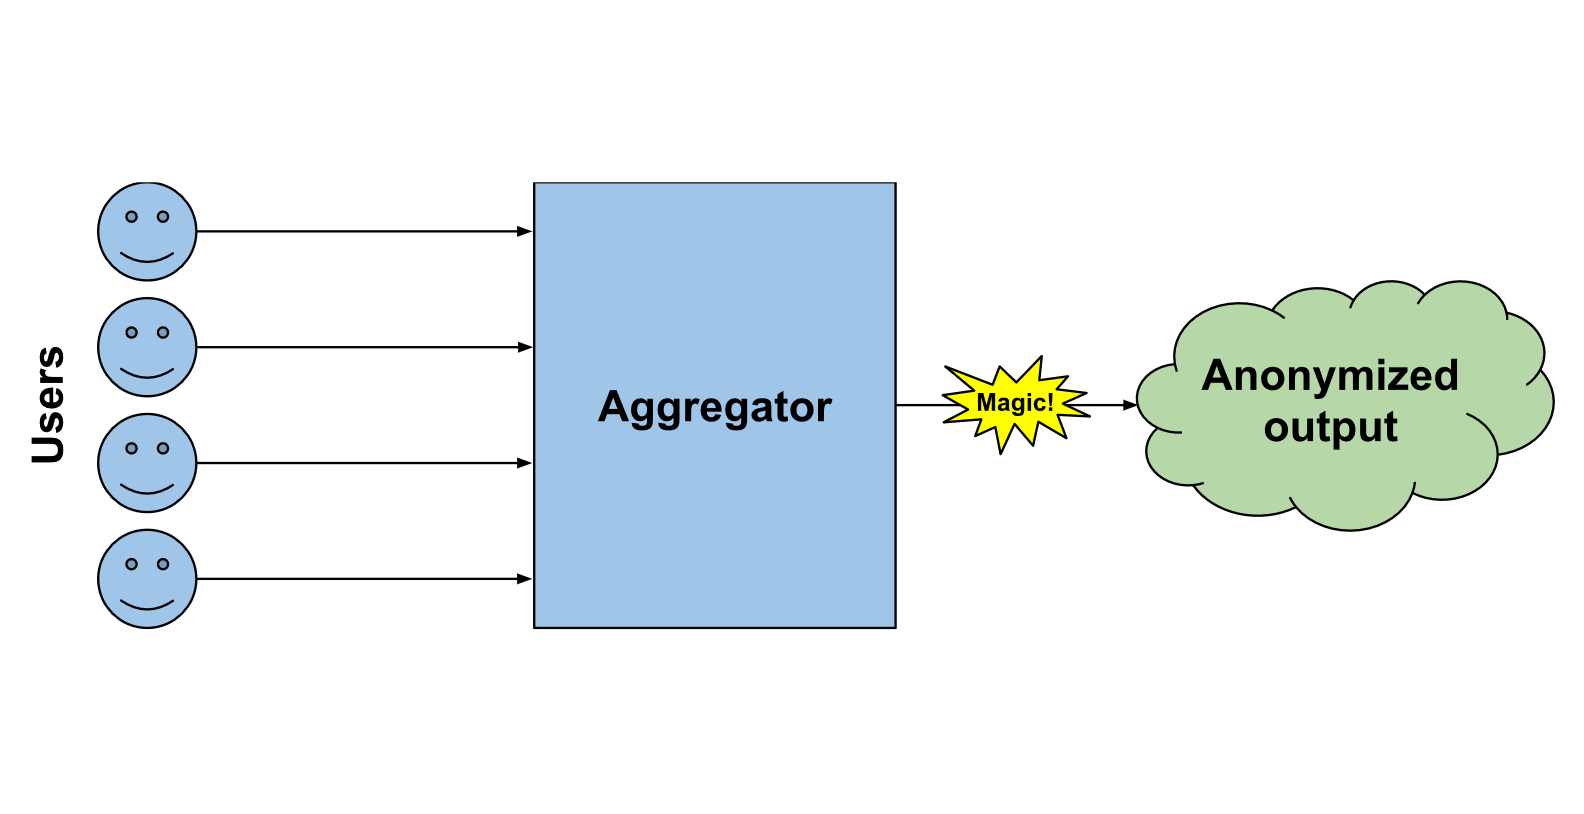
\includegraphics[width=0.8\textwidth]{figures/global_diff.png}
  \caption{Illustration of a global differential data flow\cite{desfontaines}}
  \label{fig:global_diff}
\end{figure}

\subsubsection{Local Differential Privacy}
Figure \ref{fig:local_diff} shows that differential privacy can also be used on each entry of the data. By running every entry through the mechanism, it creates a locally differential private data set. The disadvantage of this method is the much higher noise, but in exchange, the raw data itself is protected and does not require trust to an intermediate aggregator.

\begin{figure}[htpb]
  \centering
  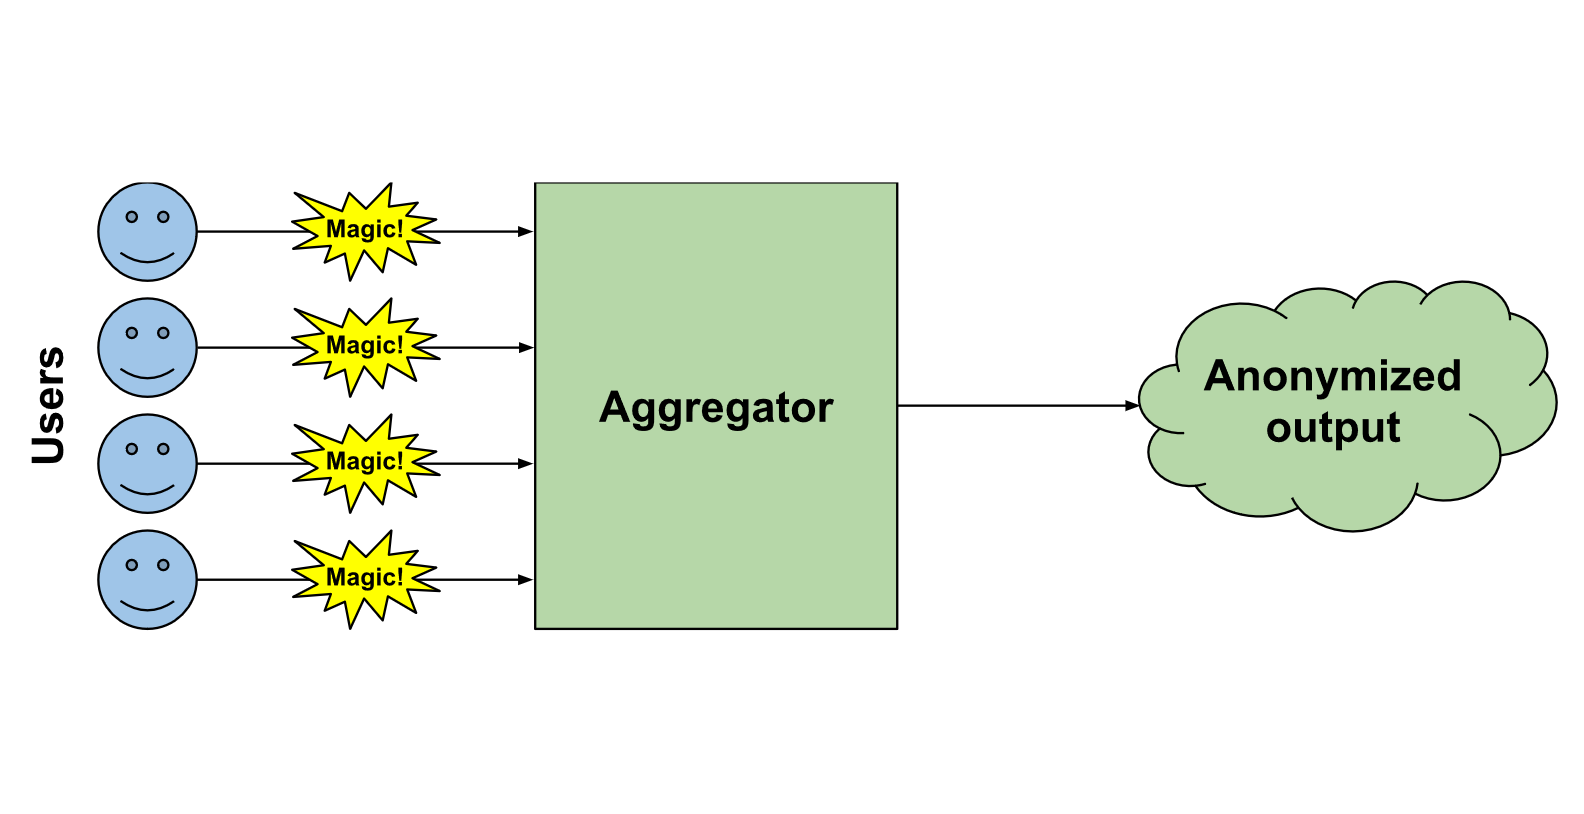
\includegraphics[width=0.8\textwidth]{figures/local_diff.png}
  \caption{Illustration of a local differential data flow \cite{desfontaines}} 
  \label{fig:local_diff}
\end{figure}

A typical example of this is the coin toss. A survey asks a question that can be answered with a yes or no. The function would toss a coin and would answer the question honestly on heads and otherwise answer the question with a second coin toss, with heads resulting in yes and tails in no. 

\subsection{Spatial Cloaking}
As mentioned above, spatial data can reveal a lot of sensitive information about a person. So location privacy should always be a high priority. Many algorithms can be used to hide the real location in a general area.

\subsubsection{Casper}
Casper \cite{DBLP:journals/tods/ChowMA09} is a grid-based cloaking mechanism that organizes the location in squares and structures the level of detail like a pyramid. It cloaks the real coordinates by using the lower-left corner and upper-right corners as a designated area of the location \cite{DBLP:conf/ssd/TanLM09}. The Figure \ref{fig:casper} would show the lowest level of detail with \(\langle(0,0),(4,4)\rangle\), covering the whole area, and the highest level of detail with \(\langle(0,2),(1,3)\rangle\), only wrapping a small portion of the area. The algorithm looks for neighboring areas for other users and then spans the whole area when it finds one to fulfill the requirements of k-anonymity. For example, \(U_1\) with its cloaked area \(\langle(0,2),(1,3)\rangle\) would need the area \(\langle(1,2),(2,3)\rangle\) to satisfy \(k=4\).

\begin{figure}[htpb]
  \centering
  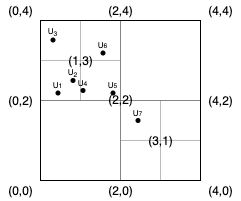
\includegraphics[width=0.5\textwidth]{figures/casper.png}
  \caption{Illustration of spatially cloaked squared areas} 
  \label{fig:casper}
\end{figure}

\subsubsection{Interval Cloaking}
Similarly to Casper, Interval Cloaking also uses rectangular cloaking areas to hide the real locations. However, instead of using neighboring squares, it uses a lower level of detail to achieve k-anonymity. Using the example from above, Interval Cloaking would span the anonymized spatial area over \(\langle(0,2),(2,4)\rangle\) to assure k-anonymity with \(k=4\) for \(U_1\) \cite{DBLP:conf/ssd/TanLM09}\cite{DBLP:conf/pet/ChengZBP06}.

\subsubsection{Hilbert Cloaking}
Another famous spatial cloaking algorithm is Hilbert Cloaking \cite{DBLP:conf/socialcom/UmKC10}. It uses the Hilbert space-filling curve to map the 2-dimensional area into a 1-dimensional representation. Then it groups together points depending on the provided \(k\) because points that are in proximity on the Hilbert curve are also close to each other in 2D. Instead of using predetermined rasterization of the area, the cloaked area is spanned by the users themselves \cite{DBLP:journals/is/GhinitaZPK10}\cite{DBLP:journals/sigkdd/Gkoulalas-DivanisKV10},\cite{DBLP:conf/ssd/TanLM09}.

% !TeX root = ../main.tex
% Add the above to each chapter to make compiling the PDF easier in some editors.

\chapter{Design}\label{chapter:design}
\section{Trust, Usability and Privacy}
In any platform, we expect a certain level of trust from each participant, may it be from the service provider or its consumer. How this trust is created can have many different sources. But the main reason a person or organization can be trusted is because of accountability. Companies with a strong market presence have the public's trust since they have been present for a longer period of time and ca not just disappear overnight
 Consequently, they can be held accountable for their actions. Today, Microsoft, Google, Amazon, and Facebook, for instance, are seen as trustworthy to a certain degree. But this trust is not invulnerable. Lies and secrecy can damage trust. Keeping the public uninformed about severe data breaches or selling sensitive data to third parties without their knowledge and permission has strained the public trust in recent years.
% Todo: \cite[Facebook Cambridge Analytica]

Even if the trust is in place, we as consumers require privacy. If we can guarantee anonymity, however, we can also guarantee privacy, as re-identification should be impossible at that point.
% Todo: \cite[Dictionary]

As chapter 2 has shown, it is a hard task to anonymize big data sets, as quasi-identifiers can be used to infer new information using linking attacks. So one way to achieve anonymity would be to strip away all attributes that could be used in another data set.

Here we hit a wall with the usability of the data itself. Cynthia Dwork says "de-identified data isn't,"
% Todo: \cite[Cynthia Dwork]
meaning that either that the data itself is not de-identified because of possible reconstruction of the data is not data anymore because it is not useful for analysis purposes. We see data itself is only as useful as its relationships.

So there is a need to find a way to find a balance between trust, usability, and privacy. Due to the limited scope of the thesis and trust being a vast research subject, we focus on the privacy of the crowd and the usability of their collected data. We assume that all participating devices and servers can be trusted, and possible adversaries only have access to the published end results.

\section{Approaches}
As mentioned before, there are advantages and disadvantages to Simon van Endern's system, and we explore how we can implement improvements and if they would be feasible with the current state of the art or if another alternative has to be chosen.

\subsection{Simon van Endern}
The proposed architecture implemented in his thesis was using a centralized approach with a distributed storage solution. The model can be seen in figure \ref{fig:simon_original}.

\begin{figure}[htpb]
  \centering
  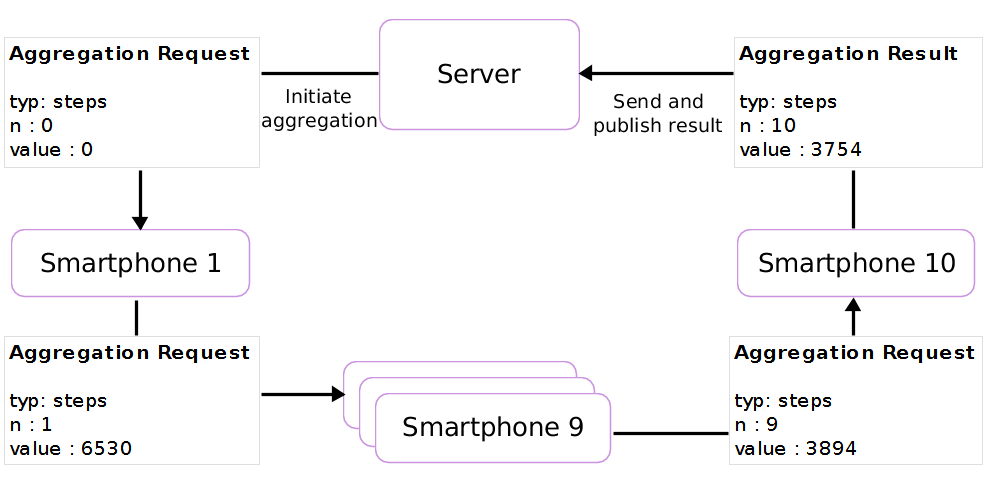
\includegraphics[width=0.8\textwidth]{figures/simon_original.png}
  \caption{Simon van Endern's original architecture.} \label{fig:simon_original}
\end{figure}

In his thesis, he eliminates the need for a central database, by collecting and storing raw data directly on the users' smartphone, creating a distributed database. This gives each participant a lot of control over their own data, just by deleting the application they are able to opt-out of future data analyses.

In his original idea, the mobile phones would use peer-to-peer technology to forward the aggregation requests and finally send the data to the server for publication. But because of the lack of available technology, he opted to use the central server as an intermediary to send from mobile phone to mobile phone. To keep the data confidential and ensure anonymity from the server, he uses RSA and AES encryption. To forward the data to the next device, he implemented a polling solution. The application periodically asks for a new aggregation request targeted at the device from the server. If one is present, it fetches the request over the REST API, and after adding its own data, it posts it back to the server targeting the next device.
In the finite scope, he managed to implement three aggregation types:

\begin{itemize}
    \item Average number of steps over the course of a day for participants. 
    \item Average time spent on an activity (walking, running, in a vehicle or on a bicycle).
    \item Average number of steps of a participant during the test period. 
\end{itemize}

We examined his work and discovered a few flaws that we might be able to improve on. We will look into possible solutions to make the architecture more efficient, scalable, secure, and privacy-preserving. 

\subsection{Expanded Approach}
Simon van Endern's original idea, as is, can hardly be scaled because of the nature of its forwarding chain. Adding \(n\) new devices creates a linear time complexity of \(\mathcal{O}(n)\) and space complexity of \(\mathcal{O}(n^2)\). For every device added, the aggregation takes up to an additional 15 minutes, and the data fetched and sent is the data of all previous devices combined, making it quite a burden on participant's data plan depending on their position in the chain.

Our first goal is to make the platform more efficient and scalable. We propose to parallelize the chains by building multiple groups for the aggregation, as shown in figure \ref{fig:aggregation}. Each chain in itself resembles the Simon van Endern's original idea in figure \ref{fig:simon_original}. With \(m\) groups, adding \(n\) devices, it only creates a time complexity of \(\mathcal{O}(\dfrac{n}{m})\) and space complexity of \(\mathcal{O}((\dfrac{n}{m})^2)\). So choosing the right \(m\) could change linear and quadratic growth to potentially constant growth. 

\begin{figure}[htpb]
  \centering
  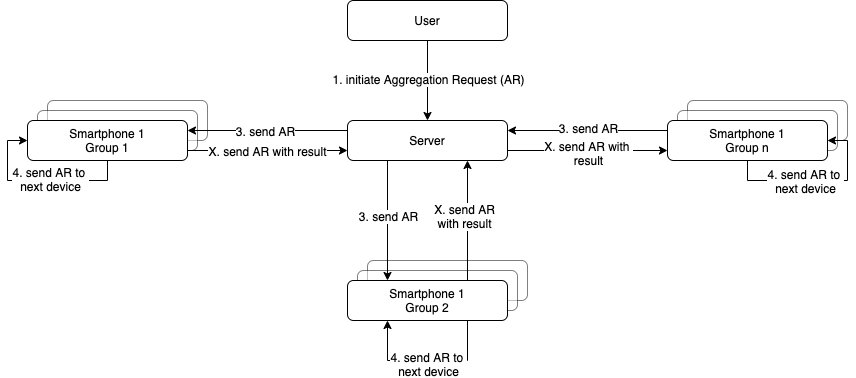
\includegraphics[width=\textwidth]{figures/aggregation}
  \caption{Distribution of still raw values.} \label{fig:aggregation}
\end{figure}

Another flaw to Simon van Endern's architecture is the constant polling for new aggregation requests. Each device periodically asks for a request targeted at it and will do so every 15 minutes. Depending on the number of participants in the project could mean up to millions of messages to the server every few minutes. To avoid this, we explore some peer-to-peer frameworks that can send data directly to the next target device and cut down on forwarding delays.

As we assume that there might possible privacy leaks, we also consider to implement local differential privacy to protect the collected data from that. We look into the benefits and the disadvantages that the implementation of this protection would bring.

Beside architectural design changes, we also want to collect more data, especially real location data. In order to extend the aggregation options, we add the two following two types:
\begin{itemize}
    \item General location of all participants in a location at a specific time
    \item Number of participants that were at a location in a specific time period
\end{itemize}


% !TeX root = ../main.tex
% Add the above to each chapter to make compiling the PDF easier in some editors.

\chapter{Implementation}\label{chapter:implementation}

The following sections describe the implementation and explain design decisions we made during development. 

\section{Technology Stack}

As our mobile platform, we have to decide between iOS and Android. While iOS has a more up-to-date operating system with 70\% of all of their mobile phones running iOS 13 and 23\% running iOS 12, Android has a much bigger market share with around 74\% compared to Apple's 25\%. 
% Todo: \cite[https://www.statista.com/statistics/272698/global-market-share-held-by-mobile-operating-systems-since-2009/]
% Todo: \cite[https://gs.statcounter.com/os-market-share/mobile/worldwide]
In terms of available development kits and libraries, both platforms provide plenty of choice. In the end, we choose Android, mainly because of their ease of deployment on devices for test scenarios and as for programming language, we opt for Kotlin instead of Java because of their intuitive syntax and compact and more readable codebase.

On the server side of development, we select Node.js using Typescript combined with MongoDB's cloud storage solution, Atlas. Node.js provides a lot of flexibility with its vast ecosystem of third party packages and MongoDB, as a NoSQL database, easily stores and combines any type of data, allowing quick changes in the data model.
% Todo: \cite[https://nodejs.org/en/]
% Todo: \cite[https://www.mongodb.com/cloud/atlas]


Our aggregation results can be fetched over the REST API or viewed directly in the MongoDB Atlas interface, given access privileges.

\section{REST API}
We use a REST API based on the JSON data exchange format and the endpoints are shown in table [X].
% Todo: insert table

The endpoints require authentication either as a researcher or as a data collecting user. For the researcher, we currently only create admin access by manually entering the username and password into the database. To register as users as a participants in the crowd, they have to send their id and their public key, as depicted in figure [X]. The server provides the participants with a random password for future authentication for sending the end result of their group.
% Todo: insert figure

\section{Aggregation API}

To start an aggregation, table [X] shows that the users have to send their \textit{username} and \textit{password} for authentication, the \textit{requestType} they wants to aggregate (steps, activity, location or presence) and additional search options as \textit{request} depending on \textit{requestType} to the server. The search options are visualized in figure [X]: 
%\begin{itemize}
%	\item \textit{start} and \textit{end} or \textit{date}, time frame or point of interest
%	\item \textit{lat} and \textit{lon}, coordinates of point of interest
%	\item \textit{radius}, distance to the point of interest
%	\item \textit{type}, type of activity as encoded in the Google Activity API
%	% Todo: \cite[https://developers.google.com/android/reference/com/google/android/gms/location/DetectedActivity.html] 
%	\item \textit{accuracy}, position after the comma to round for GPS accuracy
%	\item \textit{anonymity}, number of k-anonymity for participants
%\end{itemize}
% Todo: insert figure
% Todo: insert table for request

%\begin{figure}[h]
%\begin{multicols}{4}
%\begin{lstlisting}
%{
%	"date": 0,
%	"lat": 0,
%	"lon": 0,
%	"radius": 0
%}
%\end{lstlisting}
%\columnbreak
%\begin{lstlisting}
%{
%	"type": 0,
%	"start": 0,
%	"end": 0,
%	"lat": 0,
%	"lon": 0,
%	"radius": 0
%}
%\end{lstlisting}
%\columnbreak
%\begin{lstlisting}
%{
%	"date": 0,
%	"accuracy": 0,
%	"anonymity": 0,
%	"lat": 0,
%	"lon": 0,
%	"radius": 0
%}
%\end{lstlisting}
%\columnbreak
%\begin{lstlisting}
%{
%	"start": 0,
%	"end": 0,
%	"lat": 0,
%	"lon": 0,
%	"radius": 1
%}
%\end{lstlisting}
%\end{multicols}
%\caption{From left to right, additional information for \textit{steps}, \textit{activity},\textit{location} and \textit{presence}}
%\end{figure}

When the server receives an aggregation request of the described form, it will send out a more detailed request to the device groups for data collection. The message sent to the first mobile phones can be seen in table [X].
% Todo: insert figure
% Todo: insert table for message

After receiving and adding their data, the phones encrypt the \textit{data} JSON object and forward a similar message as figure [X] to the next device in the list. After reaching the last, it sends the results back to the server. The message to the server contains the password generated on registration for authentication.

The implementation of the different JSON formats are flexible and can accommodate more aggregation types. The next to sections will describe the process of aggregation more in depth from the Android device's and the server's point of view.

\section{Android Application}
As our target version of Android, we choose Android 10 (API level 29), which is currently the latest version of Android and as a minimum version, we select Android KitKat (API level 19). The latest report by Android shows, that around 98\% are on Android KitKat or later. To collect mobility data, we leverage the power of Google Play Services. For persistent storage, we make use of the Room Persistence Library. It provides an abstraction layer over SQLite and is commonly used in a lot of Android applications.
% Todo: \cite[https://developer.android.com/topic/libraries/architecture/room]

Because the platform relies on the generation of data from the crowd, the main functions of the application are the collection of mobility data and providing the data on request. Figure [X] describes the android applications with three main packages:
% Todo: insert figure
\begin{itemize}
	\item \textit{User Interfaces}: This package handles the start of the application and the presentation of the stored data.
	\item \textit{Background Services}: This starts all the processes in the background and manages all data and communications.
	\item \textit{Data Storage}: This part stores and fetches all the collected data.
\end{itemize}

On start up, the application opens into the \textit{Main Activity}, where it asks the users for permission to access location services. On acceptance, the application starts the background services for data collection explained in the next section. It also serves the purpose of displaying stored data in the database. A screen for each type is implemented: steps, activities and GPS. Using Simon van Endern's Android application as blueprint, we implement the same features to keep our application running behind the scenes. Because of background limitations Android introduced with Android Oreo, we create a non-dismissible notification that is displayed in the status bar and the notification center. This turns the application into a foreground application, bypassing the limitations set in the newer Android versions. To keep user interaction to a minimum, we enable the application to reopen when it crashes or is closed and when it is rebooted.

\subsection{Data Collection}
After the users successfully accepts all permissions, the \textit{Main Activity} starts the \textit{Background Service}. The \textit{Background Service} in turn starts four tasks that have been shown in figure [X]. The four modules are loosely coupled and have been separated by data type or task at hand. We split the application into data collection and data aggregation. The aggregation process will be further explained in the next section. The data collection has three modules:
\begin{itemize}
	\item \textit{Steps Service}: This module handles two classes, the step service and the step logger. If the mobile phone has a pedometer, it registers the sensor to update the step count. The step logger receives steps from the sensor and stores it in the \textit{steps\_table} ever minute. Every step entry has an \textit{start} and \textit{end} timestamp and the number of steps taken in that time frame as \textit{steps}.
	\item \textit{Activities Service}: This service, similar to the \textit{Steps Service}, is composed of the activities service and the activities logger classes. The activities service leverages the Google's Activity Recognition API to identify the current activity of the mobile device. We are only interested in the main activities: still, walking, running, on a bicycle or in a vehicle. Therefore, for all possible activities we register the transition type of entering or exiting the activity. Whenever we switch activities, the activities logger writes the \textit{timestamp}, the \textit{type} and wether we \textit{enter}ed or not into the \textit{activities\_table}. Additionally, we store the exited activity into the \textit{activitiesDetailed\_table} with the \textit{start} and \textit{end} timestamp and the \textit{type}.
% Todo: \cite[https://developers.google.com/android/reference/com/google/android/gms/location/DetectedActivity]
 	\item \textit{GPS Service}: This part of the application has the same structure as the others described above. The GPS service accesses Google's Fused Location Provider API to collect location data. The API itself uses GPS sensor as well as the network sensors in the device to determine device location. We make the location sample rate dependent on the current activity because the positional changes between \textit{still} and \textit{on a bicycle} for example are very different. So we set the interval to 5 minutes for \textit{still}, 30 seconds for \textit{walking} and 15, 5 and once per second for \textit{running}, \textit{on a bicycle} and \textit{in a vehicle} respectively. Every once in a while, the GPS logger receives batches of data from the API and saves them into the \textit{gps\_table} with their  \textit{timestamp}, \textit{lat}itude and \textit{lon}gtitude.
\end{itemize}

\subsection{Aggregation}
The last part of the background services is the \textit{Communication Service}. This is in charge of passing on data from the server or devices to the next target. For this interface we have several ideas in mind.
 
\subsubsection{IPFS}
To take out the central server as intermediary as implemented in Simon van Endern's version, we researched for libraries and SDKs that could be viable for our platform. We found the open-source projects, IPFS and libp2p, which are trying to be the foundation of the decentralized and distributed web. IPFS uses hashes to create content identifiers and turns them into blocks in a directed acyclic graph and to discover the peers with the content it uses a distributed hash table, using the modular P2P networking stack libp2p to communicate between nodes. 

Textile leverages the strength of both technologies. Their main feature is threads, a hash-chain of blocks, that can represent any type of dataset, which we could use to send data directly from device to device. Unfortunately after further investigation, the Textile SDK is not viable in its current state because it is unable to keep the node in Android alive after going into the background or turning off the device screen.

Thus we opted to instead use a third party push notification service to forward the messages between server and other devices.

\subsubsection{Push}
To replace Simon van Ender's polling with an event-based action architecture, figure [X] shows our new design. For our push service, we select Pushy
% Todo: \cite[Pushy]
% Todo: insert figure
because of their free entry version and independence from big tech companies, as well as having implementations for both iOS and Android. We could also have used Firebase Cloud Messaging to forward messages. Of course, the modular architecture of the app enables to swap this method of communication for a P2P solution as soon as one proves viable.

The complete communication infrastructure is handled by the communication service, communication receiver and communication handler. After starting the application, the \textit{Background Service} creates the communication service, that registers the device to the push service and receives a token for as identification. Then it generates a asymmetric RSA key pair and registers itself to our platform with the Pushy token as \textit{id} and the \textit{publicKey} over the REST API. As a reply, the mobile phone receives the random password for future authentication.

The communication receiver works as the entry point for push notifications from the push service and adds data to the message. Upon receiving a aggregation request like in figure [X], it checks for an encryption and if required decrypts the data field depicted in figure [X]. The application then aggregates data according to the \textit{type} sent in the \textit{requestHeader}:
\begin{itemize}
	\item \textbf{steps}: We add up the number of steps from the start and end of the specified day and add it to the list of raw values.
	\item \textbf{activities}: In this case, we sum up the time spent on the specified activity in the defined time frame and add that to the list of raw values.
	\item \textbf{location}: Here, we look for locations with the closest timestamp to the date specified in the header, but also inside a reasonable time, i.e. 10 minutes to cover the fact that still activities only logs the GPS data every 5 minutes. Then we spatially cloak the GPS coordinates and add it to the list of raw values as the hidden GPS position.
	\item \textbf{presence}: We just check all the GPS coordinates in the specified time frame, if they have been inside the range of the point of interest and add a 1 for if it has been and a 0 it hasn't.
\end{itemize}

After that, the communication handler takes the message and prepares it for the next participant in the \textit{group} array in \textit{requestOptions}. If the device was the last in the list, it sends the results to the server, otherwise it uses the hybrid encryption scheme to encrypt data with the credentials of the subsequent device. So the current device generates a symmetric AES key and encrypts the \textit{data} and afterwards does the same to the symmetric key with the public RSA key of the selected participant. Next, the communication handler forwards it over the push service, which in turn sends a push notification to the specified mobile phone.

\subsubsection{Bypassing inactive users in the aggregation chain}
In the case, that the aggregation is stuck because of any reason, for instance a device doesn't have an internet connection, it is turned off or the participant deleted the application, we have to be able to bypass the inactive mobile phone and select a new one.

With our selected push notification service, the mobile phones periodically ping the the their  server, signaling that they are online and active. Using this information, we only send aggregation requests to the participants that are marked online by the push service bypassing devices, that have been offline and haven't contacted it service in a while. But it could also be the case, that the mobile phone isn't available after the aggregation already has started.

So after the users forward their encrypted results to the following device, they start a sleeping thread, that will skip the next device and select the one after that. The subsequent user, that receives the message from the push service will aggregate the data as usual, but will send a short confirmation message back to the preceding participant, which cancels the sleeping thread. 

By avoiding offline devices and actively confirming that a request has been fulfilled, we are able to bypass inactive users and make the aggregation more efficient and reliable.

\subsubsection{Differential Privacy}

\subsubsection{Spatial Cloaking}
To be able provide k-anonymity for location data, we have to be able to generalize the GPS coordinates. By using spatial cloaking algorithms, we can hide the true position and generalize the whereabouts by assigning the user to an area. We consider using Casper, Interval Cloaking or Hilbert Cloaking. We select a variant of the Interval Cloaking algorithm  by rounding down and rounding up the digit after the comma defined in \textit{accuracy} in the \textit{requestData} to create a general rectangular area. To conserve data, we calculate the midpoint between the left lower corner and right upper corner of the area as a representative. It is important to find a good value for \textit{accuracy} because a too high value would result in a high suppression rate and too low value in too general data. 
% Todo: write about our spatial cloaking

\subsubsection{Differential Privacy}
We decide against the use of differential privacy for our use cases because of the main flaws that it provides.
\section{Server}
For our server, we are using Node.js,
% Todo: \cite[https://nodejs.org/en/]
on version 12.12.21 with the express middleware, a minimal web application framework.
% Todo: \cite[https://expressjs.com/]
Our MongoDB Atlas database instance
% Todo: \cite[https://www.mongodb.com/cloud/atlas]
receives data over the database communication module. The architecture can be seen in figure [X].
% Todo: insert figure
As our programming language, we select Typescript because of its versatility. As a superset of Javascript, it supports all Javascript libraries natively and allows for object-oriented programming paradigms. In addition, it provides optional typing and better code structure. But we transpile our Typescript code to Javascript code, to run the web server.

When we start the server, \textit{app.ts} registers the routes desribed in table [X] and connects the database object to the cloud storage instance. All calls to MongoDB are handled over that object, while the route handler manages calls to the endpoints.

\subsection{Registration}

Upon starting the application, it registers to the server using the JSON shown in figure [X] over the \textit{/crowd} route. To update the latest timestamp, we also have an obsolete route \textit{/crowd/ping}, which has been replaced with the ping our push notification service already provides. But this route can be modified to ping the devices for their current status if another communication model is adapted.

\subsection{Aggregation}

We create one routes to which the researchers can send their aggregation requests. After receiving a JSON in the mentioned form in figure [X,X,X,X] in route \textit{/aggregationRequest}, the server will get all the devices, ping them using the push service, select all the available participants and calculate the groups. Before assigning the groups, we use the Fisher-Yates shuffle to mix the order of the users. We calculate group sizes depending on a designated minimal length, so the aggregation has enough members in each group for anonymity purposes, but small enough to stay efficient. After all that, the server sends the aggregation request to all groups using the push service.

On request creation, the server creates a temporary aggregation object that stores the id, number of groups and how many it already has received. We have four additional routes for the final aggregation, \textit{/aggregationsteps}, \textit{/aggregationactivity}, \textit{/aggregationlocation} and \textit{/aggregationpresence}. They each manage the POST requests from the Android devices and calculate data or ensure anonymity.

\subsection{Anonymity}

To achieve privacy with data as sensitive as whereabouts, we use k-anonymity. For steps and activity, we don't see immediate privacy issues and thus refrain from using k-anonymity as that would needlessly lower the usability of the data without benefits. As opposed to location data, we merge the received spatially cloaked raw values and suppress all coordinates that don't fulfill the defined k. 

\section{Limitations}
Even with the proposed solutions, the architecture is still far from perfect. While the data should be confidential because of the state-of-the-art encryption, we still have to rely on a third party to deliver messages, making us dependent on their availability.

With Simon van Endern's aggregation chain, the most vulnerable participants would be the first because next in line would always be able to see the raw data they added. Unfortunately, homomorphic encryption is computationally very expensive and there are currently no available libraries for Android to implement this encryption scheme. Another possible solution would be to add dummy data for each group and remove it afterwards, so that the subsequent devices can't discern the real data of the first participant from the decoy
 data.

Another issue, that can lead to privacy issues is the centralization. While the raw data itself is distributed, the control over aggregated data, its storage and its collection is still under one central authority.
% !TeX root = ../main.tex
% Add the above to each chapter to make compiling the PDF easier in some editors.

\chapter{Performance and Evaluation}\label{chapter:evaluation}
\section{Field Test}\label{sec:field_test}
To deploy our project in the field, we used IBM Cloud's free hosting service to run our node.js server and connect it to our MongoDB, as mentioned earlier Atlas instance. We tested the system over the course of eight days from Wednesday, the 29.01.20 to Wednesday, the 05.02.20. To find participants, we asked friends, acquaintances. We tried to recruit people in the vicinity and over private social media channels. Still, unfortunately, because of privacy concerns, we only found 13 volunteers to participate in the trial, of which only 5 to 7 devices were available over the whole test period. Because of Android's own battery management system and other OEM's aggressive battery saving algorithms, a lot of devices were not reachable after they have been unused for a longer period of time, entering Doze mode. Additionally, most of our users were fragmented globally, and with the low number of active participating devices, we had to adapt our aggregation parameters. To start aggregation processes, we use Postman,
% Todo: \cite[Postman]
a tool for sending REST requests directly to an address.

We started with aggregating data specified by Simon van Endern, such as steps data and activities data, and afterward, we looked into location data and presence data. The collected data sets can be found in the Git repository
% Todo: \cite[Git repository] upload JSON
and partially in the sections below.

\subsection{Data Consumption}
Running the application by itself should not require a lot of data, as the only data consumption only comes from the initial registration request to the server, the periodical ping to the push service, and the aggregation requests. We let the application run for the first few days and aggregated data irregularly starting after the 29.01.20. But most of the requests were sent towards the end of the field test, on the 05.02.20 and the 06.02.20. In the Figure \ref{fig:diagram_requests}, the distribution of the aggregation can be seen. We were able to request proof of data consumption from 4 participants, but are only able to confirm that some of them were actively providing data in requests. The provided screenshots can be viewed in the Appendix, and consumption is shown in Table \ref{tab:data}. 

\begin{figure}[htbp]
  \centering
  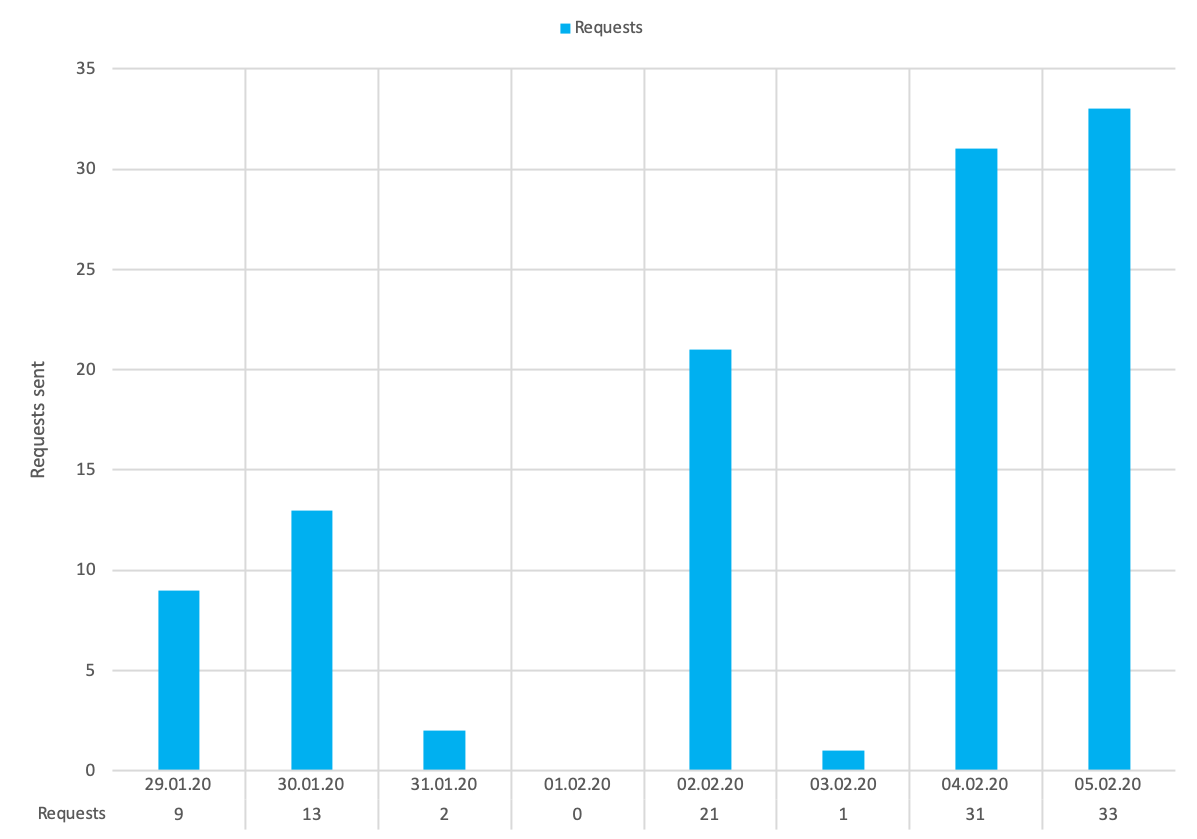
\includegraphics[width=0.8\textwidth]{figures/diagram_requests.png}
  \caption{Simon van Endern's original architecture.} \label{fig:diagram_requests}
\end{figure}

\begin{table}[htbp]
	\centering
	\begin{tabular}{|c|} 
		\hline
		\textbf{Data consumption}\\ [0.5ex] 
		\hline
		3.43 MB \\
		\hline
		3.98 MB \\
		\hline
		2.9 MB \\
		\hline
		7.89 MB \\
		\hline
	\end{tabular}
	\caption{Data consumption of devices during the test period }
	\label{tab:data}
\end{table}

We can see in all cases that data consumption did not exceed 10MB and, in most cases, did not even use more than 5MB. We could extrapolate that the consumption of data should not be a lot more than twice, depending on the number of aggregation requests sent because the parallelization of the data collection should always aim for small groups.

\subsection{Results}
We sent more than a hundred aggregation requests during the field test. We collected the average number of steps taken and the average time spent on the activities still, walking, biking, and in a vehicle. The start and end date parameters for aggregating these types were to 12:00 am JST for each day. We also requested for location and presence of the devices over the globe at 12:00 pm CET and 12:00 pm JST, 11:00 am, and 3:00 am in the GMT zone, respectively. Each aggregation had consistently from 3 to 7 participants.

% Todo: inconsistency because of the epoch time difference

We recorded the average time spent motionless was from 577 to around 1106 minutes. For individual participants, we have a wide gap with a minimum of 0 and a maximum of 1310 minutes, almost 22 hours, spent still, as depicted in Figure \ref{fig:diagram_still}. This can be explained on the basis that for counting activities, we only use finished activities that have a start and an end timestamp. For the two cases, it was highly probable that the phone has not been used touched for two full days, and thus the start date of the activity was before the 31.01.20 and the end after the 01.02.20. For the low values of 16 minutes and 28 minutes, we have not found an explanation. 

\begin{figure}[htbp]
  \centering
  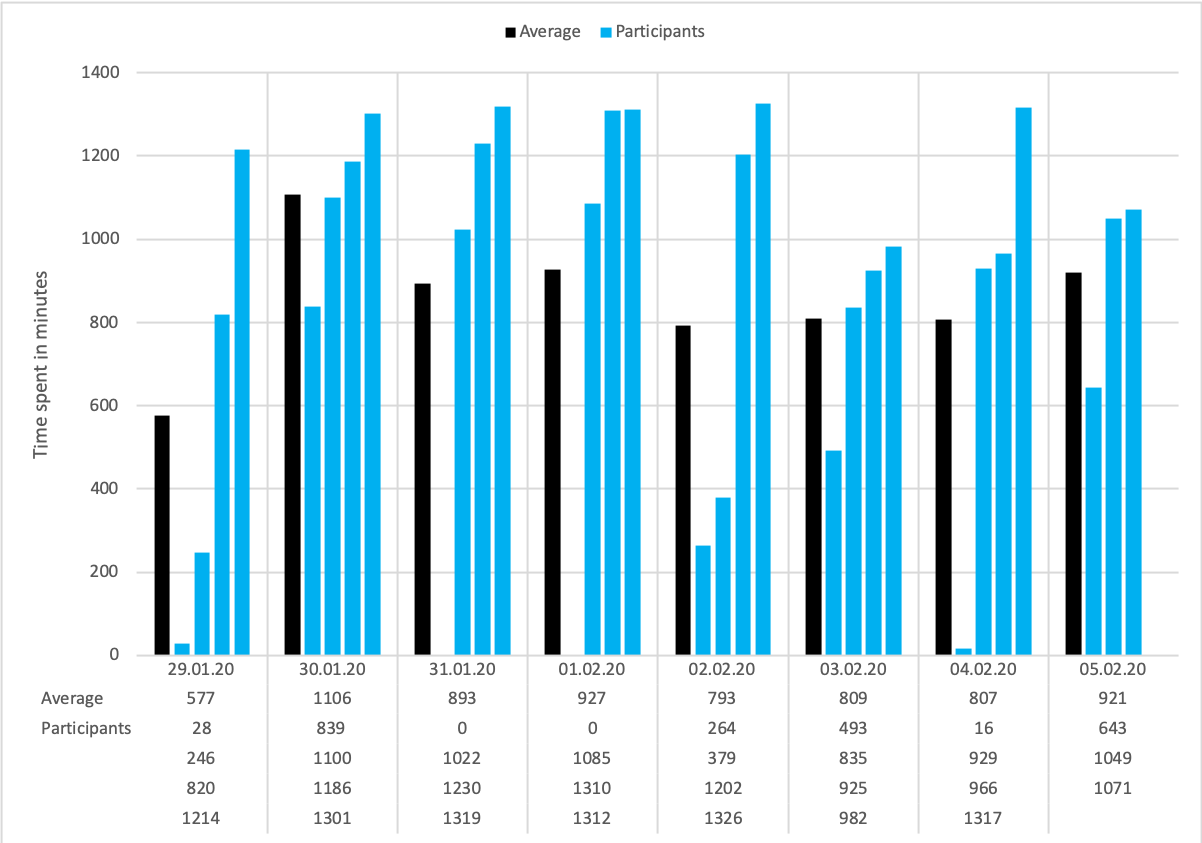
\includegraphics[width=0.8\textwidth]{figures/diagram_still}
  \caption{Distribution of still raw values.} \label{fig:diagram_still}
\end{figure}

As for walking, Figure \ref{fig:Diagram_Walking} shows a mean time between 25 and 75 minutes, from participants only walking 2 minutes up to 158 minutes. Without having the running time at hand, it is possible to infer that with the high number of steps recorded on half of the days, that one person is running regularly if the steps can be assigned to the same user.

\begin{figure}[htbp]
  \centering
  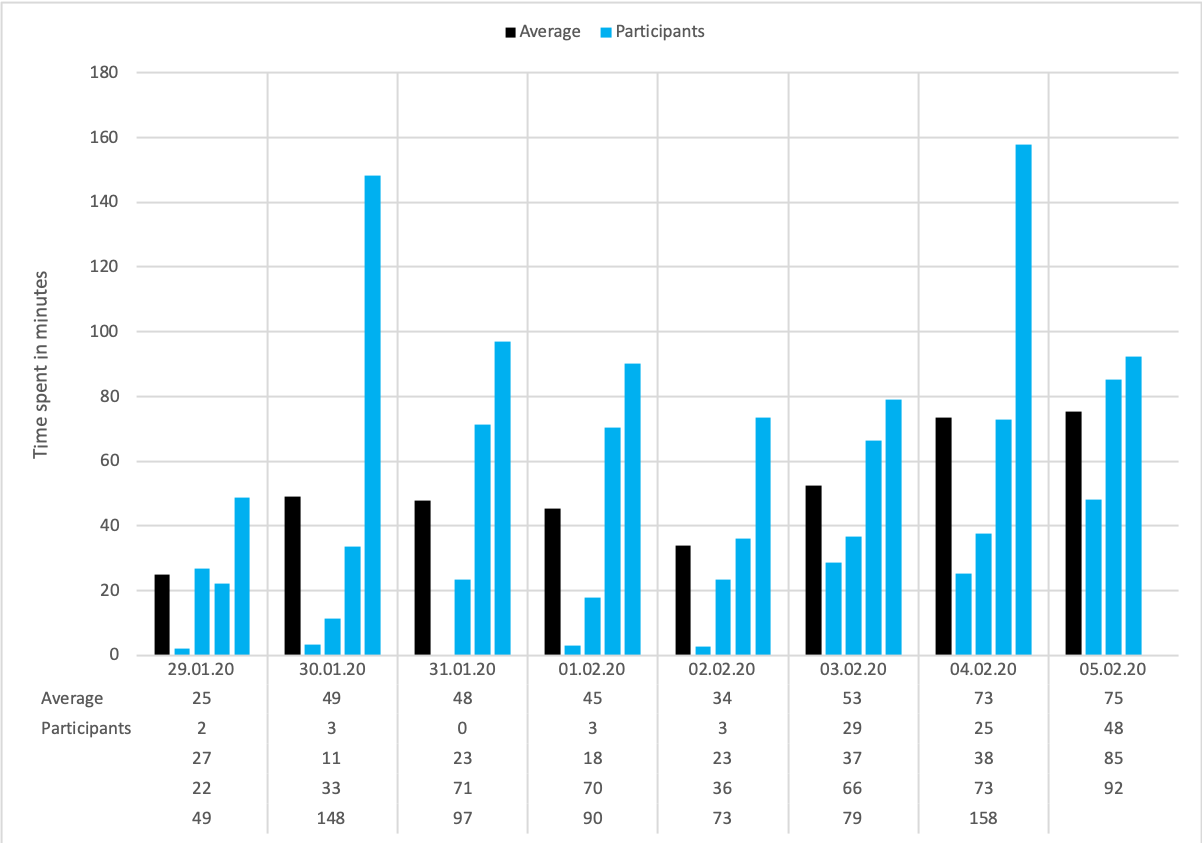
\includegraphics[width=0.8\textwidth]{figures/diagram_walking.png}
  \caption{Distribution of walking raw values.} \label{fig:diagram_walking}
\end{figure}

On average, the participant uses a vehicle for up to 106 minutes. On occasion, many users do not use any transportation at all. Figure \ref{fig:Diagram_Vehicle} shows the data a user spent in a vehicle. Registered activities from 1 to 2 minutes are with high probability credited to escalators and elevators.  

\begin{figure}[htbp]
  \centering
  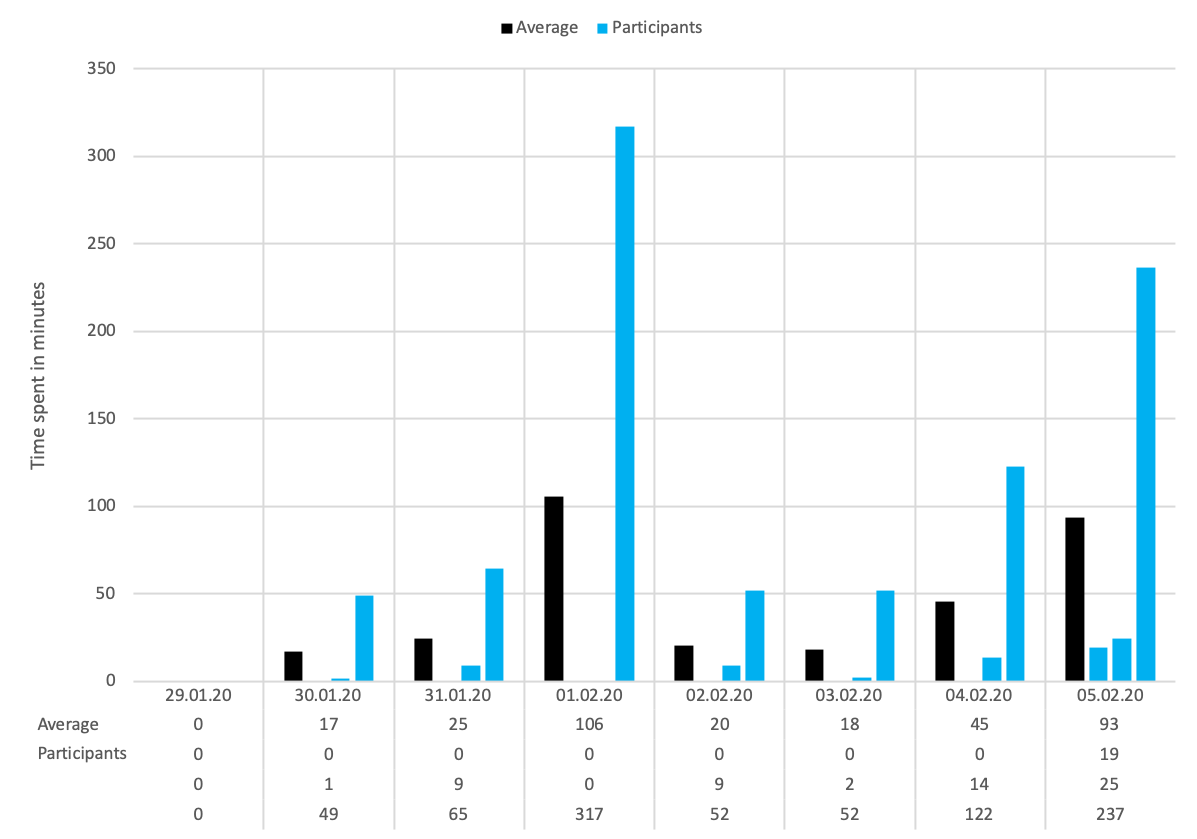
\includegraphics[width=0.8\textwidth]{figures/diagram_vehicle.png}
  \caption{Distribution of in vehicle raw values.} \label{fig:diagram_vehicle}
\end{figure}

For cycling, on some days, we only had one value of around 7 minutes. We can assume with confidence that it is one specific participant that is using the bike on occasion.

Now we take a look at the location and presence data. In the Tables \ref{tab:location_cet} and \ref{tab:location_jst}, we can see the GPS coordinates that we get after the server suppresses them for k-anonymity. We do this because there is a lot of information if only one person in a greater area is present. If we collect only spatially cloaked area in the vicinity and we do this for several time points, we can assume with high confidence, the general trajectory of that user posing a risk to privacy.

\begin{table}[htbp]
	\centering
	\begin{tabular}{|c|c|c|} 
		\hline
		\textbf{Date} & \textbf{Location} & \textbf{\# of Users} \\ [0.5ex] 
		\hline
		29.01.20 & (48.50108260577674, 11.495067909974292) & 2 \\
		&\textit{suppressed} & 1 \\
		\hline
		30.01.20 & (48.50108260577674, 11.495067909974292) & 3 \\ 
		& (35.50103138028429, 139.49688751384306) & 2 \\
		\hline
		31.01.20 & (48.50108260577674, 11.495067909974292) & 3 \\ 
		& (35.50103138028429, 139.49688751384306) & 2 \\
		\hline
		01.02.20 & (48.50108260577674, 11.495067909974292) & 2 \\ 
		\hline
		02.02.20 & (48.50108260577674, 11.495067909974292) & 2 \\ 
		& (35.50103138028429, 139.49688751384306) & 2 \\
		\hline
		03.02.20 & (48.50108260577674, 11.495067909974292) & 2 \\ 
		&\textit{suppressed} & 1 \\
		\hline
		04.02.20 & (48.50108260577674, 11.495067909974292) & 2 \\ 
		& (35.50103138028429, 139.49688751384306) & 2 \\
		&\textit{suppressed} & 1 \\
		\hline
		05.02.20 & (48.50108260577674, 11.495067909974292) & 2 \\
		&\textit{suppressed} & 2 \\
		\hline
	\end{tabular}
	\caption{Location values collected over the test period each day at 12 pm JST}
	\label{tab:location_jst}
\end{table}

\begin{table}[htbp]
	\centering
	\begin{tabular}{|c|c|c|} 
		\hline
		\textbf{Date} & \textbf{Location} & \textbf{\# of Users}\\ [0.5ex] 
		\hline
		29.01.20 &  & \\ 
		\hline
		30.01.20 &\textit{suppressed} & 2 \\ 
		& (35.50103138028429, 139.49688751384306) & 2 \\
		\hline
		31.01.20 & (48.50108260577674, 11.495067909974292) & 3 \\ 
		& (35.50103138028429, 139.49688751384306) & 2 \\
		&\textit{suppressed} & 1 \\
		\hline
		01.02.20 & (48.50108260577674, 11.495067909974292) & 3 \\ 
		& (35.50103138028429, 139.49688751384306) & 3 \\
		&\textit{suppressed} & 1 \\
		\hline
		02.02.20 & (48.50108260577674, 11.495067909974292) & 3 \\ 
		& (35.50103138028429, 139.49688751384306) & 3 \\
		&\textit{suppressed} & 1 \\
		\hline
		03.02.20 & (48.50108260577674, 11.495067909974292) & 3 \\ 
		& (35.50103138028429, 139.49688751384306) & 3 \\
		&\textit{suppressed} & 1 \\
		\hline
		04.02.20 & (48.50108260577674, 11.495067909974292) & 3 \\ 
		& (35.50103138028429, 139.49688751384306) & 3 \\
		&\textit{suppressed} & 1 \\
		\hline
		05.02.20 & (48.50108260577674, 11.495067909974292) & 2 \\ 
		\hline
	\end{tabular}
	\caption{Location values collected over the test period each day at 12 pm CET}
	\label{tab:location_cet}
\end{table}

According to the aggregated data, we have 2 to 7 participants throughout the field test. Table \ref{tab:location_jst} shows the location at 12 pm JST and Table \ref{tab:location_cet} at 12 pm CET, which corresponds to 4 am CET and 8 pm JST in the other time zone. As already mentioned before, because of the fragmented participant pool, we set the desired location at any GPS coordinates. Still, the range to 50,000km and the accuracy to 0, which results in gives us a rough estimate in a 111km range.
% Todo: \cite[GPS accuracy] 

At 12 pm JST or 4 am CET, we have only two devices located in the greater Munich area with a midpoint of \((48.50108260577674, 11.495067909974292)\) which corresponds to the territory covered by \(\langle(48, 11),(49, 12)\rangle\). On the 30th and 31st of January, we detected three devices in the same region and, additionally, 2 participants close to \((35.50103138028429, 139.49688751384306)\) which represents the space between \(\langle(35, 139),(36, 140)\rangle\). For the rest of the field test, we can determine two devices in the general area of Munich and 2 in Tokyo most of the time.

As for the aggregation at 12 pm CET or 8 pm JST, we get similar results with three devices in the greater Munich area and also three devices in the proximity of Tokyo for four days. On the 30.01.20, we only see 2 users the area covered by \(\langle(35, 139),(36, 140)\rangle\) and on the 05.02.20, we only see 2 users between \(\langle(48, 11),(49, 12)\rangle\).

Figure \ref{fig:acc0} depicts the areas that are spanned by the corner points for Munich and Tokyo. 

\begin{figure}[htbp]
  \centering
  \subfloat[Munich][Munich \(\langle(48, 11),(49, 12)\rangle\)]{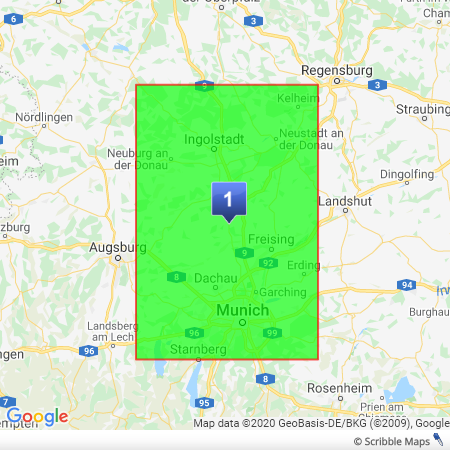
\includegraphics[width=0.45\textwidth]{figures/acc0_m}\label{fig:acc0_m}}
  \hfill
  \subfloat[Tokyo][Tokyo \(\langle(35, 139),(36, 140)\rangle\)]{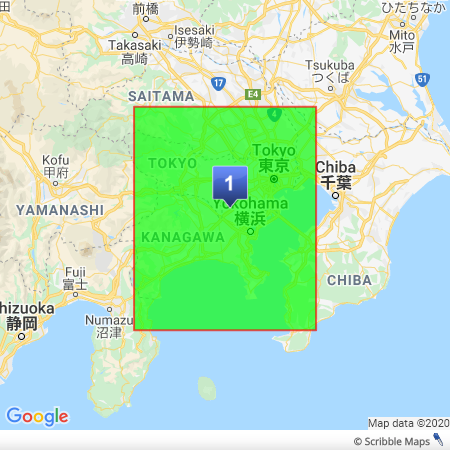
\includegraphics[width=0.45\textwidth]{figures/acc0_t}\label{fig:acc0_t}}
  \caption{Spatial areas in Tokyo and Munich with an accuracy of 0}
  \label{fig:acc0}
\end{figure}


\subsection{Privacy Evaluation}
After collecting the data, we analyze it for privacy issues. We first put the steps data and activity data under the microscope, and then we tear down the location and presence information. Examining possible reconstruction, linking, or tracing attacks.

\subsubsection{Raw Values of Steps and Activities}
Looking at the steps and the activities, we do not see any vulnerability in linking attacks as there are not a lot of possible quasi-identifiers to connect. Being able to connect temporal similarities would be a potential vulnerability. Steps data is collected over the course of the whole day, but could also be modified to use a specific time frame instead. But the issue is, that all delivered data from every device has the same time data they get from the request. The same applies to activities. As every query by itself is a statistical database, without any quasi-identifiers, it is improbable to achieve a linking attack. 
Tracing attacks, however, can be used to identify if a user is used in the query, possibly. Taking the gathered steps data, with auxiliary data as knowing the exact number of steps a person took, we can infer that the person has participated in the aggregation request with a high chance. But because our data collection architecture has a possibility that a person does not provide data, there is plausible deniability. Scaling the number of participants up, would result in a normal distribution of the mobility data, as shown by Althoff et al. With a lot of possible users, inferring the participation of one user, even with the ability to match the number of steps to exactly one value in the query result, we are unable to guarantee the user took part. We think we can assure privacy with the raw values, the same as Simon van Endern promised privacy for median values.
% Todo: \cite[Large-scale physical activity data reveal worldwide activity inequality]

\subsubsection{Location and Presence}

As for the more specific mobility data, we ca not build any connections to the other data with confidence. We are incapable of linking our location or presence to steps or activities without auxiliary data. By suppressing unique locations, that could show individuals, and we have a k-anonymous data set. But the same problems apply to it as for steps and activities. Missing quasi-identifiers make it hard to re-identify the devices that the data came from. 
But in contrast to reconstruction or linking attacks, tracing attacks could be used. Because of the lack of participating devices, we are sure that it is the same people participating in the query. But with the low accuracy, we are unable to build any trajectories. To examine the possible calculation of paths, we need more data and more accurate data.

\section{Simulated Test}
Because of the small sample size in our field test, we decided to run one more test in a more controlled environment for more reliable data. We use 10 Android Emulators on different versions of the operating system using Android Studio. We selected four small landmarks in a small area from which the devices travel from one of the other landmarks as a destination. This will ensure that we have devices that have been alone and together over the test period. For 10 minutes, each device generates location data along a predefined route in an interval of one second, totaling in 600 GPS coordinates. We use the emulator's route simulation, which leverages Google's Map API, giving us a travel speed of exactly 4.5km/h. We then aggregate the location data over the ten minutes for each minute and gather data using different accuracy parameters, giving us different approximate areas. This gives us more data to evaluate privacy issues, especially concerning historical location data.

\subsection{Results}
First, we chose an accuracy of 2 decimal places, which translates to real-world distances of around one kilometer. We were able to track 7-8 devices consistently in the areas depicted in Figure \ref{fig:acc2}. The markers 1 and 2 span the area of \(\langle(35.54, 139.63),(35.55, 139.64)\rangle\) and the other two markers are \(\langle(35.53, 139.63),(35.54, 139.64)\rangle\). Table \ref{tab:location_sim2} shows how many devices were in which area at each time step. 

\begin{table}[htbp]
	\centering
	\begin{tabular}{|c|c|c|} 
		\hline
		\textbf{Minute} & \textbf{Location} & \textbf{\# of Users}\\ [0.5ex] 
		\hline
		1 & (35.54500010319573, 139.63499968824985) & 4 \\ 
		& (35.535000103183386, 139.63499968836484) & 4 \\ 
		&\textit{suppressed} & 2 \\ 
		\hline
		2 & (35.54500010319573, 139.63499968824985) & 4 \\ 
		& (35.535000103183386, 139.63499968836484) & 3 \\ 
		&\textit{suppressed} & 3 \\ 
		\hline
		3 & (35.54500010319573, 139.63499968824985) & 3 \\ 
		& (35.535000103183386, 139.63499968836484) & 4 \\ 
		&\textit{suppressed} & 3 \\ 
		\hline
		4 & (35.54500010319573, 139.63499968824985) & 3 \\ 
		& (35.535000103183386, 139.63499968836484) & 4 \\ 
		&\textit{suppressed} & 3 \\ 
		\hline
		5 & (35.54500010319573, 139.63499968824985) & 3 \\ 
		& (35.535000103183386, 139.63499968836484) & 4 \\ 
		&\textit{suppressed} & 3 \\ 
		\hline
		6 & (35.54500010319573, 139.63499968824985) & 4 \\ 
		& (35.535000103183386, 139.63499968836484) & 4 \\ 
		&\textit{suppressed} & 2 \\ 
		\hline
		7 & (35.54500010319573, 139.63499968824985) & 4 \\ 
		& (35.535000103183386, 139.63499968836484) & 4 \\ 
		&\textit{suppressed} & 2 \\ 
		\hline
		8 & (35.54500010319573, 139.63499968824985) & 4 \\ 
		& (35.535000103183386, 139.63499968836484) & 4 \\ 
		&\textit{suppressed} & 2 \\  
		\hline
		9 & (35.54500010319573, 139.63499968824985) & 4 \\ 
		& (35.535000103183386, 139.63499968836484) & 4 \\ 
		&\textit{suppressed} & 2 \\ 
		\hline
		10 & (35.54500010319573, 139.63499968824985) & 3 \\ 
		& (35.535000103183386, 139.63499968836484) & 4 \\ 
		&\textit{suppressed} & 3 \\ 
		\hline
	\end{tabular}
	\caption{Location values collected over the simulated test period for each minute with an accuracy of 2}
	\label{tab:location_sim2}
\end{table}

\begin{figure}[htbp]
  \centering
  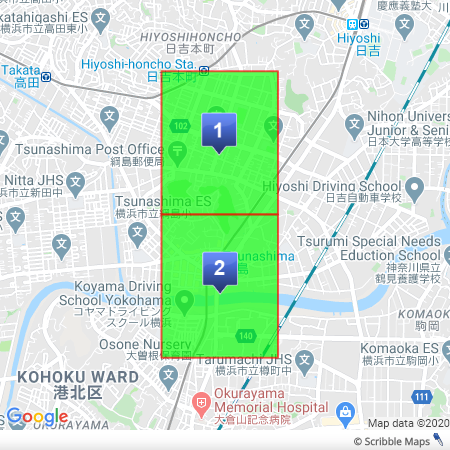
\includegraphics[width=0.5\textwidth]{figures/acc2}
  \caption{Spatially cloaked areas for an accuracy value of 2} \label{fig:acc2}
\end{figure}

Because the region we specified is large, we can almost always find multiple devices in the area.

\begin{figure}[htbp]
  \centering
  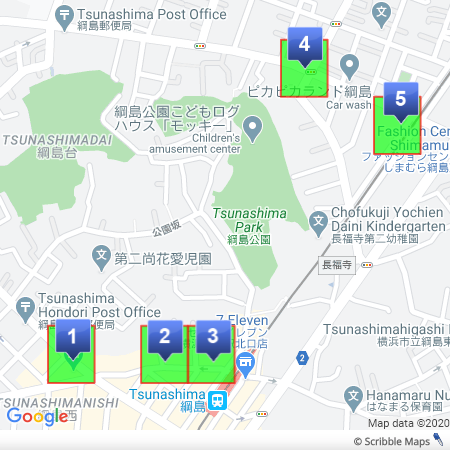
\includegraphics[width=0.5\textwidth]{figures/acc3}
  \caption{Spatially cloaked areas for an accuracy value of 3} \label{fig:acc3}
\end{figure}

For our next aggregation, we selected a precision of 3, which corresponds to roughly 100 meters. The data in Table \ref{tab:location_sim3} reveals that we can find two mobile phones most of the time, with aggregations, in which we were able to find three devices or none at all. The areas are visible in Figure \ref{fig:acc3}.

\begin{table}[htbp]
	\centering
	\begin{tabular}{|c|c|c|} 
		\hline
		\textbf{Minute} & \textbf{Location} & \textbf{\# of Users}\\ [0.5ex] 
		\hline
		1 & (35.537500001031866, 139.63149999688338) & 2 \\ 
		&\textit{suppressed} & 8 \\ 
		\hline
		2 & (35.537500001031866, 139.63149999688338) & 2 \\ 
		&\textit{suppressed} & 8 \\ 
		\hline
		3 & (35.537500001031866, 139.6334999968834) & 2 \\ 
		&\textit{suppressed} & 8 \\ 
		\hline
		4 & \textit{suppressed} & 10 \\
		\hline
		5 & (35.537500001031866, 139.63449999688333) & 2 \\ 
		&\textit{suppressed} & 8 \\ 
		\hline
		6 & (35.537500001031866, 139.63549999688334) & 2 \\ 
		& (35.54250000103193, 139.6364999968828) & 2 \\ 
		&\textit{suppressed} & 6\\
		\hline
		7 & (35.537500001031866, 139.63549999688334) & 3 \\ 
		& (35.54150000103191, 139.6384999968829) & 2 \\ 
		&\textit{suppressed} & 5\\ 
		\hline
		8 & (35.537500001031866, 139.63549999688334) & 2 \\ 
		&\textit{suppressed} & 8 \\ 
		\hline
		9 & (35.537500001031866, 139.63449999688333) & 2 \\ 
		&\textit{suppressed} & 8 \\ 
		\hline
		10 & (35.537500001031866, 139.63549999688334) & 2 \\ 
		&\textit{suppressed} & 8 \\ 
		\hline
	\end{tabular}
	\caption{Location values collected over the simulated test period for each minute with an accuracy of 3}
	\label{tab:location_sim3}
\end{table}

Finally, we send requests with an accuracy of 4 or 10 meters. In this scenario, we were almost unable to register any devices, except for minute 10, see Table \ref{tab:location_sim4}. At this time point, we have two users that pass each other in \(\langle(35.5372, 139.6336),(35.5373, 139.6337)\rangle\) as seen in Figure \ref{fig:acc4}.

\begin{table}[htbp]
	\centering
	\begin{tabular}{|c|c|c|} 
		\hline
		\textbf{Minute} & \textbf{Location} & \textbf{\# of Users}\\ [0.5ex] 
		\hline
		1 & \textit{suppressed} & 10 \\
		\hline
		2 &\textit{suppressed} & 10 \\
		\hline
		3 &\textit{suppressed} & 10 \\
		\hline
		4 &\textit{suppressed} & 10 \\
		\hline
		5 &\textit{suppressed} & 10 \\
		\hline
		6 &\textit{suppressed} & 10 \\
		\hline
		7 &\textit{suppressed} & 10 \\
		\hline
		8 &\textit{suppressed} & 10 \\
		\hline
		9 &\textit{suppressed} & 10 \\
		\hline
		10 & (35.53725000001032, 139.63364999996884) & 2 \\ 
		&\textit{suppressed} & 8 \\ 
		\hline
	\end{tabular}
	\caption{Location values collected over the simulated test period for each minute with an accuracy of 4}
	\label{tab:location_sim4}
\end{table}

\begin{figure}[htbp]
  \centering
  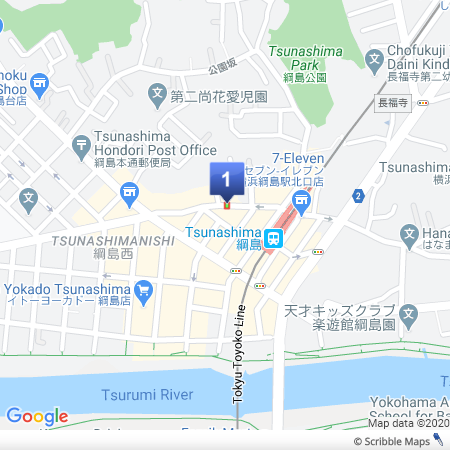
\includegraphics[width=0.5\textwidth]{figures/acc4}
  \caption{Spatially cloaked areas for an accuracy value of 4} \label{fig:acc4}
\end{figure}

\subsection{Privacy Evaluation}
Looking at the documented results, we can see where devices meet each other. With low precision, we always register 3-4 users. Using k-anonymity, we are unable to find out more than the provided data. We only know the number of people present in a specific area. 

After we increased precision to 3, we mostly see pairs. According to the Table \ref{tab:location_sim3}, in the first 3 minutes, we can assume that two devices pass each other in the same area. Later, one of them leaves the zone, and we stop registering that region. Without auxiliary information, we are unable to find out in which direction the users traveled or who left the area first. In minute 5 to 9, we register two adjacent regions. We can assume that there are more than two phones in the vicinity. Analyzing the historical spatial data, we suggest that we have two devices in area 2 and one device in zone 3 at minute 5. In the sixth minute, we register a new domain and loose the old one, indicating that one device moved from region 2 to 3 while the other two are still in their respective areas. In minute 9, we then see the old area again and the new one vanishing, suggesting that the device that was formerly in area 3 walked into zone 2. We are able to infer the travel direction of one device, but are still unable to point out the device.

Using an accuracy of 10 meters, we are unable to collect any useful data. The lack of devices in such a small area resulted in mostly suppressed data.  

\subsection{Usability}
By stripping away all of the quasi-identifiers, we sacrifice a lot of possible usability in the data. But for the loss of value, we are able to preserve a lot of privacy and even provide anonymity. On the one hand, we will not be able to use the collected data for detailed medical research that requires sex, age, and other information. On the other hand, however, we can gather population density data and activity data, which are very handy in urban planning. This provides a good starting point to find a balance between the usability of data and the privacy of the data provider.

\subsection{Possible Improvements}
We achieved a lot of scalability and a lot of privacy in our implementation, but there are still immediate improvements possible in both the application and the server. For the spatially cloaked location data, our design only applies static accuracy provided by the request itself. It may be possible to send different accuracies of the concealed areas and match them on the server, to get smaller anonymizing regions and, at the same time, still maintain k-anonymity.

The application should also be tweaked to be able to handle multiple requests at the same time. It is thus making data aggregation, in general, more efficient. The same applies to the server. At the moment, it does not differentiate the messages it receives from the groups. It is forcing researchers to wait for an aggregation to finish before they are able to send a new request.

As homomorphic encryption is still in its infancy, an alternative to protect the first participants from the subsequent is to add dummy data that can be removed at the end. This method would hide the primary data added to the aggregation and make it harder for the second device in the chain to determine the real input from the fake.

We also have an issue with the confirmation approach. This method is right now implemented using a sleeping thread that prepares to resend the data collected so far to the subsequent device after time out, but which in turn creates another sleeping thread. It may lead to multiple threads that use a lot of resources and might cause the application to freeze or crash.


% !TeX root = ../main.tex
% Add the above to each chapter to make compiling the PDF easier in some editors.

\chapter{Conclusion}\label{chapter:conclusion}
While it is hard to strike a balance between anonymity and usability, we think we found a starting point on which we can build for a more scalable, secure, and privacy-preserving platform for collecting, aggregating, and analyzing of mobility data.

\section{Research Questions}
\subsection*{RQ1: What are the benefits and drawbacks in van Endern's architecture and what improvements are possible?}
After examination, we found that van Endern managed to collect a lot of data while preserving privacy. Additionally, his idea provided a very secure communication infrastructure using a hybrid encryption scheme. His proposal, however, wasn't able to scale because of it, creating long wait times for data collection.
Furthermore, the single aggregation chain leads to to a quadratic growth in data consumption, and our current data plans are unable to carry that burden. On the upside, the lone series of collection hides the connection between the data and the device. On the downside, his implementation of forwarding requests using a polling system over HTTPS creates a drain on the battery.
Another flaw in the design is the selection process of the next device. Giving the server the ability to choose the following target allows it to choose compromised users and to endanger their privacy. 

In chapter 3, we proposed a few upgrades and extended the data collection. To help aggregation, we changed the polling mechanism to a straightforward event-driven one. Using a third-party push notification service, we are able to send requests directly to the participating mobile phones instead of giving them the job to fetch the requests from the server, improving significantly on communication time. We also suggested splitting the single aggregation chain into multiple groups, creating several smaller series of devices to collect the data instead of one long one, parallelizing the process, and cutting down on collection time. We also added the ability to request more accurate mobility data, such as the raw values of steps and activities and information about the location of devices or the presence of a device at a location. 

\subsection*{RQ3: What information do the raw values for steps and activities reveal?}
We added raw values to the aggregation of steps and activities as we saw no infraction on privacy by providing these values if there are enough participants. It is crucial to expand the number of users to a certain number to provide privacy because as long as the numbers are low, we can trace the contribution of a participant in an aggregation. At a certain point, the steps and activities data should take the form of a uniform distribution, which then hides the individual raw data inside the collected data set. When that number of participants is reached and the inability to determine if a user participated in the collection request, we are confident that the privacy of the participants is secure. A side-effect that also helps protect privacy is the uncertainty of participation because of the distributed storage of raw data. We are unable to identify if a device played a part in the result or not.

\subsection*{RQ4: How much information does the aggregation of real location data expose?}
We found that similar to other types of data, the number of participants is vital to protect their identity or at least their association. Using suppression, we are unable to hide devices, that are on their own. In chapter 5, we tested the platform in the field and a controlled setting. We were unable to draw any reliable conclusions regarding the usability of the collected data because of the lack of participants in our deployed field test. Regarding privacy, however, we don't see any way how the data can be used to infer more sensitive data or even identity. The spatial cloaking mechanism successfully hides the real location of the devices while revealing interesting statistical data. In the simulated test, we were able to collect much more reliable data. We were able to deduce the travel direction of one unidentified device but were unable to trace it back to other information.

\subsection*{RQ5: Can we use the current state of peer-to-peer technology to remove intermediate third parties?}
Chapter 4 has shown our attempt to implement peer-to-peer technology into a mobile application. We have identified Textile as a viable candidate for our project, but unfortunately, one of the most important aspects didn't meet our expectations. There is a lot of progress in that aspect of technology, but some work still has to be done before it can be used in production. We should also look into decentralized communication standards, such as matrix \cite{matrix}, that can be used as an alternative to our initial direct communication approach.

\section{Limitations}
As mentioned before, there are a lot of short-term obstacles that we identified that could be improved and some that warrant further research in the long-term.

First, both our field test and simulated test were executed on a very limited number of devices, giving us only a glimpse into our solution for scalability and privacy. The number of participants in an aggregation request can range from a few people in a rural area to a few thousand or even a few million in crowded metropoles. Further tests should be performed to collect a more extensive data set, but we expect them to confirm our assumptions.

Second, for the sake of the scope of the thesis, we assumed that the server and the mobile devices are trusted, and a malicious actor only has access to the aggregated data set. But for further research, the possibility of a compromised server and/or compromised mobile phones must be taken into consideration. Given an untrusted server, it is able to view the groups and its participants and the data received from each group. We have suspicions that the server would be able to connect the values sent to the mobile device it was sent from by resending the same request multiple times and observing the changes in the grouped collection. In case that there are compromised participants, the integrity of the data is in danger. The privacy of some devices might be jeopardized, but we believe that the mixed groups sent from the server would create enough randomness so that the malicious devices won't be able to build a profile. In the event that the server and participants are malicious, we aren't able to guarantee any protection.

\section{Future Work}
We have shown that the work we have done looks very promising, but a lot of issues were left untouched because of the limited constraints of the thesis. Below, we suggest a few subjects that could be considered in the future. 

\subsection{Mobile}
The biggest extension would be to implement the mobile application for iOS platform. This opens up questions to cross-platform or native development. Furthermore, the Apple App Store has a lot of restrictions regarding the privacy and could eventually hinder the deployment. But creating the application for the iOS platform opens up more participants, resulting in more data for research.

With the trend in decentralization, peer-to-peer technology is being developed hand-in-hand by many organizations. Being able to communicate with the next devices directly, instead of involving an intermediary, will cut out on possible points of failure and provide a more secure communication channel.

As discussed in the earlier chapters, homomorphic encryption could be an excellent tool to keep data confidential while enabling arithmetic operations on them. Using this method allows for the calculation of values without knowing the raw data, preventing sensitive information from prying eyes. This technology might not pertain to privacy and anonymity directly but would still make the platform more secure.

Another technique to strengthen privacy would be to give the users the control to participate in the data collection themselves. An option in which they can decide what level of privacy the collected data holds. I.e., either setting the collection to very private, so that all data gathered with the option is protected from aggregation or just changing the privacy level of the data itself.

Also mentioned in the section above is that trust is a topic that can't be handled lightly. Either intentionally providing false information or trying to trace or link private data to a device are possible motives for a malicious user. To combat misinformation and privacy leaks, there has to be a way to establish trust. Pouryazdan et al. \cite{DBLP:journals/access/PouryazdanKSFS17} suggest a score to measure the reputation, which in our eyes could either help with data reliability or create a new quasi-identifier for adversaries to exploit.
 
\subsection{Server}
Trust is also an issue for the server. With scandals constantly being reported on, the public trust in corporations and organizations collecting sensitive data is waning. Establishing the server as a trustworthy instance that doesn't mishandle the collected data by enhancing privacy or guaranteeing anonymity would be a step in the right direction. Relinquishing control over the data from a centralized architecture into a decentralized one would be an even bigger step and give the users more protection.

\subsection{Blockchain}
Leveraging the power of blockchain, the platform can incentivize the user to participate in aggregation. Ming et al. [X] suggest CrowdBC, a decentralized framework for crowdsourcing using blockchain. 

On the one hand, compensating the crowd for participating on the platform would result in more data collected. On the other hand, however, the existence of monetary value would draw in the attention of malicious intentions, making it hard for data to be trustworthy.

\section{Reproducibility}
Further research on the collection, aggregation, and analysis of mobility data with the use of a scalable, secure, and privacy-preserving platform can be done using our implementation. In the README file
% Todo: \cite[README]
, we noted down instructions for the installation and local deployment of the server. The necessary tools for the setup are also documented. Comments in the code will indicate the places additional changes, such as API keys for the push notification service and URLs for the push notification server and the database instance, have to be added to run it correctly. As for storage, we built the platform with MongoDB's cloud solution in mind, so utilizing an alternative might require changes to the database module. Section \ref{sec:field_test} shows the deployment option we used, but the server can be hosted on any platform, and the database could be deployed locally.

On the client-side, we have mobile phones. The application can be built using the Android Studio IDE and installed on any compatible Android device. Similar to the server, the comments specify the locations where URLs have to be modified. The application was built from the ground up with modularity in mind, making it possible to replace communication schemes.
% Todo: \cite[application]

First, the server and the database has to be running. After that, the Android applications can be started, triggering the registration process automatically when the permissions have been accepted. With everything online, aggregation requests can be initiated by consuming the REST API detailed in section \ref{sec:api}, and the end result should be stored in the deployed database instance.


% !TeX root = ../main.tex
% Add the above to each chapter to make compiling the PDF easier in some editors.

\chapter{Introduction}\label{chapter:xx01introduction}
Use with pdfLaTeX and Biber.

\section{Section}
Citation test (with Biber)~\parencite{latex}.

\subsection{Subsection}  
See~\autoref{tab:sample}, \autoref{fig:sample-drawing}, \autoref{fig:sample-plot}, \autoref{fig:sample-listing}, \autoref{fig:tum}, \autoref{fig:tumslide}.

\begin{table}[htpb]
  \caption[Example table]{An example for a simple table.}\label{tab:sample}
  \centering
  \begin{tabular}{l l l l}
    \toprule
      A & B & C & D \\
    \midrule
      1 & 2 & 1 & 2 \\
      2 & 3 & 2 & 3 \\
    \bottomrule
  \end{tabular}
\end{table}

\begin{figure}[htpb]
  \centering
  % This should probably go into a file in figures/
  \begin{tikzpicture}[node distance=3cm]
    \node (R0) {$R_1$};
    \node (R1) [right of=R0] {$R_2$};
    \node (R2) [below of=R1] {$R_4$};
    \node (R3) [below of=R0] {$R_3$};
    \node (R4) [right of=R1] {$R_5$};

    \path[every node]
      (R0) edge (R1)
      (R0) edge (R3)
      (R3) edge (R2)
      (R2) edge (R1)
      (R1) edge (R4);
  \end{tikzpicture}
  \caption[Example drawing]{An example for a simple drawing.}\label{fig:sample-drawing}
\end{figure}

\begin{figure}[htpb]
  \centering

  \pgfplotstableset{col sep=&, row sep=\\}
  % This should probably go into a file in data/
  \pgfplotstableread{
    a & b    \\
    1 & 1000 \\
    2 & 1500 \\
    3 & 1600 \\
  }\exampleA
  \pgfplotstableread{
    a & b    \\
    1 & 1200 \\
    2 & 800 \\
    3 & 1400 \\
  }\exampleB
  % This should probably go into a file in figures/
  \begin{tikzpicture}
    \begin{axis}[
        ymin=0,
        legend style={legend pos=south east},
        grid,
        thick,
        ylabel=Y,
        xlabel=X
      ]
      \addplot table[x=a, y=b]{\exampleA};
      \addlegendentry{Example A};
      \addplot table[x=a, y=b]{\exampleB};
      \addlegendentry{Example B};
    \end{axis}
  \end{tikzpicture}
  \caption[Example plot]{An example for a simple plot.}\label{fig:sample-plot}
\end{figure}

\begin{figure}[htpb]
  \centering
  \begin{tabular}{c}
  \begin{lstlisting}[language=SQL]
    SELECT * FROM tbl WHERE tbl.str = "str"
  \end{lstlisting}
  \end{tabular}
  \caption[Example listing]{An example for a source code listing.}\label{fig:sample-listing}
\end{figure}

\begin{figure}[htpb]
  \centering
  
\includegraphics[width=0.8\textwidth]{tum}
  \caption[Something else can be written here for listing this, otherwise the caption will be written!]{Includegraphics searches for the filename without extension first in logos, then in figures.} \label{fig:tum}
\end{figure}

\begin{figure}[htpb]
  \centering
  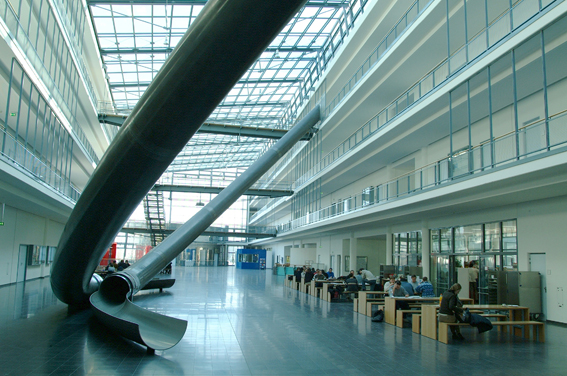
\includegraphics[width=0.8\textwidth]{figures/tum}
  \caption{For pictures with the same name, the direct folder needs to be chosen.} \label{fig:tumslide}
\end{figure}

\begin{figure}[!tbp]
  \centering
  \subfloat[TUM Logo][The logo.]{
\includegraphics[height=0.2\textheight]{tum}\label{fig:tum1}}
  \hfill
  \subfloat[TUM Slide][The famous slide.]{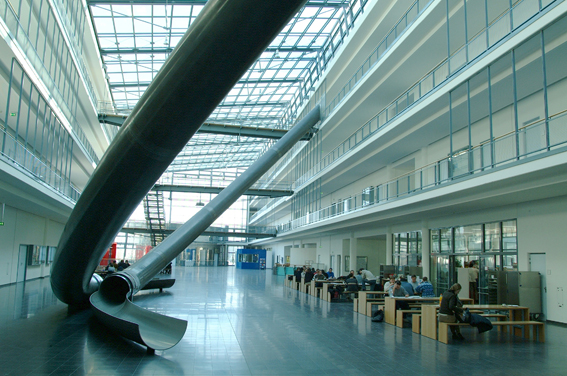
\includegraphics[height=0.2\textheight]{figures/tum}\label{fig:tum2}}
  \caption{Two TUM pictures side by side.}
  \label{fig:sidebyside}
\end{figure}

This is how the glossary will be used.

\Glspl{ddye}, \gls{r0}, \gls{R0}, and \gls{kdeac}. Also, the \glspl{tum} has many \glspl{computer}, not only one \Gls{computer}. Subsequent acronym usage will only print the short version of \glspl{tuma} (take care of plural, if needed!), like here with \gls{tuma}, too. It can also be --> \glsdisp{tum}{hidden}\footnote{Example for a hidden TUM glossary entry.} <--.

\todo{Now it is your turn to write your thesis.

This will be a few tough weeks.}

\done{Nevertheless, celebrate it when it is done!}

% TODO: add more chapters here

\chapter{Second Introduction}\label{chapter:second_introduction}
Use with pdfLaTeX and Biber.


\appendix{}

% TODO: appendix chapter
\chapter{General Addenda}

If there are several additions you want to add, but they do not fit into the thesis itself, they belong here.

\section{Detailed Addition}

Even sections are possible, but usually only used for several elements in, e.g.\ tables, images, etc.

\chapter{Figures}
\section{Example 1}
\cmark
\section{Example 2}
\xmark

\microtypesetup{protrusion=false}
\listoffigures{}
\listoftables{}
\microtypesetup{protrusion=true}
\printglossaries
\printbibliography{}

\end{document}
